% Generated by Sphinx.
\documentclass[a4wide,10pt,italian]{manual}
\usepackage[utf8]{inputenc}
\usepackage[T1]{fontenc}
\usepackage{babel}
\usepackage{times}
\usepackage[Sonny]{fncychap}
\usepackage{longtable}
\usepackage{sphinx}
\usepackage{fancyhdr}
\pagestyle{fancy}

\title{SANET - rilascio di un prodotto per il monitoraggio delle reti}
\date{05 Dicembre 2009 \\ Questo documento è rilasciato con licenza CC-BY-SA 3.0}
\author{Luca Ferroni \\ Laboratori Guglielmo Marconi S.p.A.}
\newcommand{\sphinxlogo}{}
\renewcommand{\releasename}{Release}
\makeindex

\newcommand\PYGZat{@}
\newcommand\PYGZlb{[}
\newcommand\PYGZrb{]}
\newcommand\PYGaz[1]{\textcolor[rgb]{0.00,0.63,0.00}{#1}}
\newcommand\PYGax[1]{\textcolor[rgb]{0.84,0.33,0.22}{\textbf{#1}}}
\newcommand\PYGay[1]{\textcolor[rgb]{0.00,0.44,0.13}{\textbf{#1}}}
\newcommand\PYGar[1]{\textcolor[rgb]{0.73,0.38,0.84}{#1}}
\newcommand\PYGas[1]{\textcolor[rgb]{0.25,0.44,0.63}{\textit{#1}}}
\newcommand\PYGap[1]{\textcolor[rgb]{0.00,0.44,0.13}{\textbf{#1}}}
\newcommand\PYGaq[1]{\textcolor[rgb]{0.38,0.68,0.84}{#1}}
\newcommand\PYGav[1]{\textcolor[rgb]{0.00,0.44,0.13}{\textbf{#1}}}
\newcommand\PYGaw[1]{\textcolor[rgb]{0.13,0.50,0.31}{#1}}
\newcommand\PYGat[1]{\textcolor[rgb]{0.73,0.38,0.84}{#1}}
\newcommand\PYGau[1]{\textcolor[rgb]{0.32,0.47,0.09}{#1}}
\newcommand\PYGaj[1]{\textcolor[rgb]{0.00,0.44,0.13}{#1}}
\newcommand\PYGak[1]{\textcolor[rgb]{0.14,0.33,0.53}{#1}}
\newcommand\PYGah[1]{\textcolor[rgb]{0.00,0.13,0.44}{\textbf{#1}}}
\newcommand\PYGai[1]{\textcolor[rgb]{0.73,0.38,0.84}{#1}}
\newcommand\PYGan[1]{\textcolor[rgb]{0.13,0.50,0.31}{#1}}
\newcommand\PYGao[1]{\textcolor[rgb]{0.25,0.44,0.63}{\textbf{#1}}}
\newcommand\PYGal[1]{\textcolor[rgb]{0.00,0.44,0.13}{\textbf{#1}}}
\newcommand\PYGam[1]{\textbf{#1}}
\newcommand\PYGab[1]{\textit{#1}}
\newcommand\PYGac[1]{\textcolor[rgb]{0.25,0.44,0.63}{#1}}
\newcommand\PYGaa[1]{\textcolor[rgb]{0.19,0.19,0.19}{#1}}
\newcommand\PYGaf[1]{\textcolor[rgb]{0.25,0.50,0.56}{\textit{#1}}}
\newcommand\PYGag[1]{\textcolor[rgb]{0.13,0.50,0.31}{#1}}
\newcommand\PYGad[1]{\textcolor[rgb]{0.00,0.25,0.82}{#1}}
\newcommand\PYGae[1]{\textcolor[rgb]{0.13,0.50,0.31}{#1}}
\newcommand\PYGaZ[1]{\textcolor[rgb]{0.25,0.44,0.63}{#1}}
\newcommand\PYGbf[1]{\textcolor[rgb]{0.00,0.44,0.13}{#1}}
\newcommand\PYGaX[1]{\textcolor[rgb]{0.25,0.44,0.63}{#1}}
\newcommand\PYGaY[1]{\textcolor[rgb]{0.00,0.44,0.13}{#1}}
\newcommand\PYGbc[1]{\textcolor[rgb]{0.78,0.36,0.04}{#1}}
\newcommand\PYGbb[1]{\textcolor[rgb]{0.00,0.00,0.50}{\textbf{#1}}}
\newcommand\PYGba[1]{\textcolor[rgb]{0.02,0.16,0.45}{\textbf{#1}}}
\newcommand\PYGaR[1]{\textcolor[rgb]{0.25,0.44,0.63}{#1}}
\newcommand\PYGaS[1]{\textcolor[rgb]{0.13,0.50,0.31}{#1}}
\newcommand\PYGaP[1]{\textcolor[rgb]{0.05,0.52,0.71}{\textbf{#1}}}
\newcommand\PYGaQ[1]{\textcolor[rgb]{0.78,0.36,0.04}{\textbf{#1}}}
\newcommand\PYGaV[1]{\textcolor[rgb]{0.25,0.50,0.56}{\textit{#1}}}
\newcommand\PYGaW[1]{\textcolor[rgb]{0.05,0.52,0.71}{\textbf{#1}}}
\newcommand\PYGaT[1]{\textcolor[rgb]{0.73,0.38,0.84}{#1}}
\newcommand\PYGaU[1]{\textcolor[rgb]{0.13,0.50,0.31}{#1}}
\newcommand\PYGaJ[1]{\textcolor[rgb]{0.56,0.13,0.00}{#1}}
\newcommand\PYGaK[1]{\textcolor[rgb]{0.25,0.44,0.63}{#1}}
\newcommand\PYGaH[1]{\textcolor[rgb]{0.50,0.00,0.50}{\textbf{#1}}}
\newcommand\PYGaI[1]{\fcolorbox[rgb]{1.00,0.00,0.00}{1,1,1}{#1}}
\newcommand\PYGaN[1]{\textcolor[rgb]{0.73,0.73,0.73}{#1}}
\newcommand\PYGaO[1]{\textcolor[rgb]{0.00,0.44,0.13}{#1}}
\newcommand\PYGaL[1]{\textcolor[rgb]{0.02,0.16,0.49}{#1}}
\newcommand\PYGaM[1]{\colorbox[rgb]{1.00,0.94,0.94}{\textcolor[rgb]{0.25,0.50,0.56}{#1}}}
\newcommand\PYGaB[1]{\textcolor[rgb]{0.25,0.44,0.63}{#1}}
\newcommand\PYGaC[1]{\textcolor[rgb]{0.33,0.33,0.33}{\textbf{#1}}}
\newcommand\PYGaA[1]{\textcolor[rgb]{0.00,0.44,0.13}{#1}}
\newcommand\PYGaF[1]{\textcolor[rgb]{0.63,0.00,0.00}{#1}}
\newcommand\PYGaG[1]{\textcolor[rgb]{1.00,0.00,0.00}{#1}}
\newcommand\PYGaD[1]{\textcolor[rgb]{0.00,0.44,0.13}{\textbf{#1}}}
\newcommand\PYGaE[1]{\textcolor[rgb]{0.25,0.50,0.56}{\textit{#1}}}
\newcommand\PYGbg[1]{\textcolor[rgb]{0.44,0.63,0.82}{\textit{#1}}}
\newcommand\PYGbe[1]{\textcolor[rgb]{0.40,0.40,0.40}{#1}}
\newcommand\PYGbd[1]{\textcolor[rgb]{0.25,0.44,0.63}{#1}}
\newcommand\PYGbh[1]{\textcolor[rgb]{0.00,0.44,0.13}{\textbf{#1}}}
\begin{document}
\shorthandoff{"}
\maketitle
\tableofcontents

\lhead[SANET - rilascio di un prodotto per il monitoraggio delle reti]{\scalebox{0.500000}{
\includegraphics{by-sa.png}} Luca Ferroni}
\rhead[Luca Ferroni \scalebox{0.500000}{
\includegraphics{by-sa.png}}]{SANET - rilascio di un prodotto per il monitoraggio delle reti}

\chapter{Introduzione}

SANET è l'acronimo di Security Architecture NETwork
ed è il software di monitoraggio per le reti sviluppato da
Laboratori Guglielmo Marconi S.p.A. (LABS) a partire dal 2006.

Il 12 giugno 2009 SANET è stato rilasciato da LABS con la licenza di software libero AGPLv3
alla pagina \href{http://sanet.sourceforge.net}{http://sanet.sourceforge.net}.

In questo documento si illustra il processo che ha portato alla
realizzazione di SANET, le motivazioni del progetto, gli obiettivi che raggiunge,
le fasi di sviluppo e le decisioni relative al rilascio come software libero.

Non si intende scrivere un manuale utente del software. Installazione ed utilizzo
sono descritte nella documentazione online. Per una panoramica del software con le sue peculiarità
rimandiamo all'articolo di presentazione scritto per la CONFSL09 e pubblicato nel sito di SANET.

In particolare relativamente al rilascio della seconda versione
viene mostrato il lavoro svolto nella \textbf{rappresentazione della mappe topologiche della rete}
e il \textbf{processo di pacchettizzazione} avviato per facilitare l'installazione del software ad utenti meno
esperti di sistemi.

Il tutto è concluso da una verifica del lavoro svolto e possibili future direzioni,
sia dal punto di vista tecnico, sia di approccio alla comunità.

In appendice viene riservato uno spazio con:
\begin{itemize}
\item {} 
una analisi sulla sicurezza del software

\item {} 
una mail girata nella mailing-list cisco-nsp che presenta alcuni aspetti tecnici avanzati soddisfatti da SANET

\item {} 
l'analisi comparativa effettuata nella scelta fra le tecnologie SVG e FLASH.

\end{itemize}

Buona lettura

\resetcurrentobjects
\hypertarget{--doc-context}{}

\chapter{In quale contesto nasce l'idea di SANET ?}

In questo capitolo vedremo in quale contesto nasce SANET.
Quando si è deciso di svilupparlo, chi lo ha deciso.

Cosa si è voluto realizzare e da cosa si è partiti,
e perché è stato avviato un nuovo progetto evitando di
adattare un programma open source esistente alle proprie esigenze.


\section{Chi}

LABS è un'azienda che si occupa di reti. Segue il processo di messa in funzione di una rete
a partire dalla progettazione dell'infrastruttura fisica, per poi passare al livello rete,
fino ad arrivare ai servizi.

Il cosiddetto \emph{core business} dei LABS è l'assistenza sulle reti. Le reti hanno bisogno
di monitoraggio e manutenzione continui e in reti complesse non si può fare a meno
di avere tecnici specializzati per risolvere le più disparate problematiche che si presentano.

I problemi si possono verificare ad esempio a causa di:
\begin{itemize}
\item {} 
retaggi del passato

\item {} 
deperimento dell'hardware

\item {} 
cause estemporanee (ad esempio bachi in aggiornamenti software oppure gestione \href{http://www.meinberg.de/english/info/leap-second.htm}{ntp leap second} ?)

\item {} 
worm/attacchi nella rete

\end{itemize}


\section{Da cosa si parte}

Il sistema di monitoraggio preesistente prendeva il nome di \emph{pinger} ed era un monolitico script in Perl
che disponeva di un linguaggio per la definizione dei controlli.

Il linguaggio era abbastanza basilare, ma consentiva di definire modelli abbastanza comodi
per istruire il sistema su una serie di controlli da effettuare.

Il pregio di questo software consisteva proprio nella definizione duttile e dettagliata dei parametri
da verificare per ogni controllo: a quali intervalli di tempo effettuarli,
per quale soglia di tolleranza e a chi veicolare le segnalazioni.
Tutto ciò in un modo relativamente semplice.

I difetti invece si possono riassumere in:
\begin{itemize}
\item {} 
incomprensibilità dei risultati dell'attività di monitoraggio per il cliente

\item {} 
interfaccia grafica pressoché inesistente

\item {} 
caricamento in memoria di tutti i controlli da effettuare e riavvio del software in caso di modifica della configurazione

\item {} 
mancanza di \emph{escalation} ossia di dipendenza dei controlli e quindi flood di allarmi per un unico problema

\item {} 
limitazioni varie dovute alla ridotta espressività del linguaggio e del parsing dello stesso

\item {} 
multiprocesso, ma non multithread con conseguente sovraccarico di memoria

\item {} 
parsing dei controlli non resistente a \emph{code injection}

\end{itemize}

È da notare che il tutto si è sempre basato su GNU/Linux e strumenti open source
e anche la realizzazione stessa rimaneva open: i clienti più smaliziati potevano
andare a curiosare nel codice e suggerire modifiche oltre ovviamente a definire i propri controlli.

Tuttavia non si può dire che questa situazione fosse ben definita, dato che, di fatto \emph{pinger} era da sempre
installato su appliance LABS e LABS stesso non ha mai esplicitato la licenza dello strumento in quanto
era funzionale al servizio di assistenza delle reti che diveniva oggetto principale del contratto con il cliente.

Da questa considerazione si può desumere che LABS è sempre stato autore più o meno consapevole di software open,
ma non aveva ancora tenuto in considerazione la possibilità di condividere apertamente la propria
conoscenza, di creare una comunità intorno all'attività di monitoraggio delle reti che ha da sempre costituito
un punto di eccellenza per l'azienda.

Ciò ovviamente era anche dovuto all'assenza di un settore di sviluppo software e quindi al modo \emph{artigianale}
in cui veniva sviluppato \emph{pinger}. Per capire basta sapere che il versionamento del software avveniva tramite
\emph{diff} e \emph{patch} ... che, a onor del vero, lo stesso Linus Torvalds ritiene un meccanismo ben più evoluto di CVS
(si veda il video \href{http://www.youtube.com/watch?v=4XpnKHJAok8}{Linus Torvalds on Git}), ma che comunque rasenta la definizione di
versionamento.

In ultimo è necessario osservare che LABS stava avviando in quel periodo una piccola divisione di sviluppo software
per portare avanti altri progetti.


\section{L'esigenza}

Le doti del sistema di monitoraggio in uso erano confermate dai casi di successo riscontrati
presso i clienti LABS che tipicamente hanno sempre presentato
infrastrutture di rete mediamente o molto complesse.

Da qui si è deciso di intraprendere una nuova strada, o meglio, di consolidare la strada già intrapresa:
reingegnerizzare il sistema di monitoraggio valorizzandone i pregi, superandone i limiti e colmandone le lacune.

Si sa che nello sviluppo software ``l'appetito vien mangiando'' e, anche se non si aveva l'ambizione
di realizzare il software di monitoraggio perfetto,
si è capito che ristrutturando quello che già c'era a disposizione
si sarebbe potuto:
\begin{itemize}
\item {} 
soddisfare nuove esigenze

\item {} 
ottenere uno strumento più facile da mantenere ed estendere

\item {} 
potenziare l'espressività e la tassonomia dei controlli da effettuare

\item {} 
adattarsi o integrare nuove tecnologie

\end{itemize}

Non a caso la \textbf{soddisfazione} di nuove esigenze \textbf{del cliente*+ è stata elencata al primo posto:
questa **è la motivazione che spinge le aziende a investire e innovare}.

Anche nel caso dei LABS, sebbene le motivazioni fossero molteplici, il momento dell'investimento,
il cosiddetto \emph{trigger} è stata la richiesta sempre più insistente di un'interfaccia grafica
comprensibile: il cliente lamentava di non essere consapevole in alcun modo della situazione della propria rete
e che le informazioni estremamente dettagliate e tecniche fornite dalla scarna interfaccia di \emph{pinger}
non fossero per lui di alcuna utilità.

Quindi la decisione è stata di aprire gli orizzonti, coinvolgere il gruppo di sviluppatori,
e progettare un software per il monitoraggio delle reti che superasse i limiti di \emph{pinger}
(con priorità per i limiti di rappresentazione grafica dei risultati),
mantenesse il know-how pluriennale dell'azienda e anche il proprio \emph{modus operandi}.

Trattandosi questa volta di un software vero e proprio più che di un insieme di script
si inizia a valutare la possibilità di rilasciare il lavoro alla comunità.
In azienda il terreno è fertile: si comprende l'importanza di condividere conoscenza,
la ricchezza del servizio, della cultura e della prestazione professionale
invece che il valore artificioso della licenza centellinata
e pure si coglie marginalmente il vantaggio reciproco (per l'azienda a la comunità) che ne sarebbe potuto derivare.

La strada del software libero non è già tracciata, ma inizia a diffondersi nell'aria.
Un merito che bisogna dare ai LABS è che continuando con contratti sul servizio di assistenza alle reti,
non sarebbe sussistito alcun obbligo di rilascio del software:
infatti tale software non sarebbe stato ceduto al cliente, ma sarebbe rimasto
uno strumento di proprietà dell'azienda per offrire il servizio concordato.
Inoltre la presentazione dei risultati sarebbe avvenuta tramite interfaccia web
e quindi anche in questo caso si sarebbe rimasti nel pieno della legittimità
a meno di integrare software basato su licenza \href{http://www.fsf.org}{Affero GPLv3} o
con simili requisiti a tutela di libertà per l'utente.


\section{Quando}

Il lavoro di analisi, definizione obiettivi e progettazione della nuova architettura è
iniziato nel 2005.

I più diffusi sistemi open source esistenti per il monitoraggio delle reti erano già
conosciuti dagli esperti di rete LABS e non si è ritenuto opportuno fare un'approfondita valutazione
di integrabilità con l'esistente.

In quel periodo \href{http://zenoss.org}{ZenOSS} , uno dei progetti open source più frequentati
su \href{http://sourceforge.net}{SourceForge.net} e più attivi al momento della scrittura di questo documento,
non era ancora stato avviato.

Quindi, considerando anche l'ampia base di controlli sviluppati dall'azienda, i casi di successo riscontrati
e le modalità operative assodate, ci si è diretti verso lo sviluppo di una nuova soluzione,
accettando in questo modo di non approfittare di comunità già consolidate sui temi del network management.

Questa scelta ha ovviamente avuto un impatto decisivo sull'impostazione dello sviluppo della nuova piattaforma
che voleva a questo punto evolvere dalla precedente senza rompere con il passato per continuare appunto,
a consolidare la strada già intrapresa.

Si presentava lo scenario di rimpiazzare l'auto in corsa: non interrompere il servizio, ma sostituire gradualmente parti
di software migliorandone gradualmente la qualità complessiva.

\resetcurrentobjects
\hypertarget{--doc-development}{}

\chapter{Le fasi di sviluppo}

Evolvere un programma che porta con se i retaggi di un passato decennale
oltre che l'approccio prettamente pratico del sistemista non è un percorso semplice,
soprattutto se si intende reingegnerizzare il tutto in modo da minimizzare la rottura
con il passato e farne un software manutenibile in cui sia chiara la separazione delle componenti.

Si decide di partire con lo sviluppo di \emph{SANET}.


\hypertarget{first-attempt-failed}{}\section{Un primo tentativo fallito}

In principio si è approcciato il problema in modo abbastanza superficiale:
presa coscienza delle parti da sostituire, si è scelto il linguaggio Python già
in uso nell'azienda per altri progetti e si è demandata la prima stesura del nuovo codice
ad un collaboratore temporaneo.

Questo approccio si è dimostrato fallimentare perché:
\begin{itemize}
\item {} 
aveva l'ambizione di sostituire in breve tempo tutta la vecchia piattaforma

\item {} 
non si appoggiava ad alcun framework che potesse velocizzare lo sviluppo focalizzando l'attenzione
sulle peculiarità di SANET

\item {} 
basava la sua implementazione su uno storage in memoria e anche qui ne é derivata una perdita di tempo
ed energie in problemi di concorrenza e persistenza delle informazioni

\item {} 
si voleva implementare una politica di ereditarietà molto complessa fra istanze madri, categorie,
e istanze collegate: in pratica si stava riscrivendo un linguaggio a oggetti

\end{itemize}

e inoltre non possiamo trascurare che dal punto implementativo queste sfide erano state
sottovalutate dall'azienda che non ha dedicato risorse umane per seguire costantemente
il collaboratore temporaneo che si è trovato probabilmente smarrito con in mano un linguaggio
di programmazione che non conosceva e problematiche che non aveva mai affrontato dal punto
di vista pratico.


\section{Fase 0: una migrazione graduale}

Una volta che la collaborazione temporanea è terminata, le persone coinvolte nel progetto
si sono confrontate e, considerata la situazione, si è scelto di far tesoro dell'esperienza
fatta, salvare il salvabile (che comunque non era trascurabile) e partire per una migrazione
più graduale.

Si è pensato di appoggiarsi ad un RDBMS per la memorizzazione persistente dei dati, la gestione
dell'atomicità e dell'isolamento delle interazioni, la coerenza dei dati (in quest'ordine
proprietà DAIC di solito note come ACID !).

Inoltre avvalersi di un backend DB che sfruttasse il linguaggio SQL per l'interazione,
avrebbe consentito in modo semplice di adattare le parti scritte in Perl man mano
che la nuova implementazione in Python procedeva.

Vediamo quali fasi si sono susseguite nello sviluppo di SANET.


\section{Fase 1: Django + RDBMS}

\textbf{Obiettivo visualizzazione}: sfruttare le nuove tecnologie web per realizzare una
interfaccia ricca (RIA) che potesse essere fruibile da vari browser e pertanto
non richiedesse di essere installata su ogni postazione.

Da una disamina degli \emph{application server} disponibili per Python si è scelto il nuovo
framework Django che pure era solamente alla versione 0.96.
Si è subito deciso di adottare la versione SVN che disponeva di funzionalità molto più
avanzate della versione rilasciata e avrebbe dato anche la possibiltà di segnalare patch
e essere sincronizzati con la comunità di sviluppatori.

Fra i pregi che hanno contribuito alla scelta:
\begin{itemize}
\item {} 
è basato su pattern modello-vista-template (\href{http://docs.djangoproject.com/en/dev/faq/general/\#django-appears-to-be-a-mvc-framework-but-you-call-the-controller-the-view-and-the-view-the-template-how-come-you-don-t-use-the-standard-names}{MTV}, una interpretazione del più comune \href{http://en.wikipedia.org/wiki/Model\%E2\%80\%93view\%E2\%80\%93controller}{MVC} )

\item {} 
è indipendente da un particolare backend DB: all'inizio si è usato MySQL ma poco dopo si è passati a PostgreSQL.
Si voleva lasciare aperta già in principio questa possibilità date esperienze precedenti non troppo soddisfacenti
con MySQL

\item {} 
come dicono gli sviluppatori: Django è Python ! Non ci sono vincoli particolari da rispettare,
o imponenti infrastrutture da costruire (come ad esempio accade in Zope). Inoltre il sistema è veramente molto
duttile e si può decidere di utilizzare solamente una componente (ad esempio soltanto il modello come poi avviene con la CLI)

\end{itemize}

Lo \emph{application server} è scelto e pertanto viene relegata ad esso
una serie importante di problematiche di basso livello come:
\begin{itemize}
\item {} 
interazione con RDBMS

\item {} 
interazione con socket

\item {} 
parsing delle richieste HTTP

\item {} 
serializzazione delle risposte HTTP

\item {} 
astrazione del backend autenticazione: ogni infrastruttura di rete dispone di propri meccanismi

\end{itemize}

A questo punto si è definito il modello dei dati che verrà popolato dall'attività di monitoraggio
di \emph{pinger} (riadattato per l'esigenza): questi saranno i dati visualizzati nell'interfaccia web.


\subsection{INIL, SITEATTR, FOREST}

Il database è stato progettato in 3 parti logicamente suddivise:
\begin{itemize}
\item {} 
INIL (icon, node, interface, link): contiene le tabelle base che
rappresentano la topologia della rete e le icone. In questa parte
rientrano anche le configurazioni dei controlli, sebbene l'acronimo non le comprenda

\item {} 
SITEATTR (siteattr): contiene una tabella con il registro globale di configurazione del
sito (nome, ultima modifica, numero di thread, etc.)

\item {} 
FOREST: (tree, container, node\_tree\_pos): contiene le tabelle per
rappresentare alberi di contenitori, e per posizionare i nodi nei contenitori..

\end{itemize}

Nella prima fase l'implementazione di INIL si è concentrata sulle
tabelle contenenti le informazioni di configurazione e di stato dei controlli. Per quello che riguarda
i nodi e le interfacce di rete si è pensato di inserire solo le informazioni anagrafiche indispensabili
alla rappresentazione, mentre i link sono stati totalmente relegati al momento dell'implementazione futura delle mappe topologiche.

Realizzare SITEATTR è stato ovviamente banale una volta deciso di memorizzare queste informazioni
nel database è bastato dedicare una tabella con parametri e valori globali all'applicazione.

La parte FOREST è totalmente nuova rispetto a \emph{pinger} e si è deciso di realizzarla subito.
Essa è risultata di fondamentale importanza per catalogare le risorse della rete e quindi offrire all'utente
viste specializzate dell'ambiente monitorato.

I contenitori sono strutturati ad albero in modo analogo alle directory strutturate nella gerarchia del file system. In questa metafora è come se i nodi di rete fossero i file da catalogare nelle directory. In SANET tuttavia l'espressività della categorizzazione è maggiore rispetto a quella del file system in quanto un nodo di rete può essere associato a diversi contenitori che non appartengono allo stesso albero.
Ogni albero identifica una tipologia di categorizzazione e i contenitori una specifica categoria. Alberi comunemente usati sono relativi alla dislocazione geografica degli apparati, alla gerarchia di responsabilità, o ancora alla tipologia dei nodi di rete in esso contenuti.
Classificare un nodo di rete in contenitori di alberi diversi in SANET significa applicare quei concetti di tag o categorizzazione duttile tipici delle \href{http://en.wikipedia.org/wiki/Folksonomy}{folksonomie del Web 2.0}.

Considerando che ogni pagina di SANET è la rappresentazione di ciò che è contenuto nella risorsa selezionata,
usare in modo corretto i contenitori consente di offrire ad utenti specifici cruscotti, che di solito prendono
il nome inglese di \emph{dashboard},  tramite i quali osservare l'andamento delle risorse di rete di propria responsabilità
o comunque le risorse di proprio interesse.


\subsection{SANET visualizza lo stato della rete}

Come risultato di questa fase viene soddisfatta la prima priorità: visualizzare lo stato della rete in modo comprensibile
all'utente medio. Una svolta epocale per i LABS: da questo momento non sarebbero stati solo i tecnici ad avere
visibilità totale e ``macchinosa'' degli eventi, ma tutti avrebbero avuto un'idea delle problematiche
o quantomeno avrebbero saputo di qualcosa che non stava funzionando nel modo atteso.

...e anche di dove ciò stava accadendo: SANET infatti fin dalla prima versione
implementa il meccanismo dei contenitori che era totalmente assente nel sistema precedente.

\emph{Pinger} nel contempo era stato adattato all'interazione con lo RDBMS e continuava ad essere eseguito con le seguenti mansioni:
\begin{itemize}
\item {} 
interpretazione della configurazione per i controlli

\item {} 
monitoraggio: verifica dello stato e aggiornamento misurazioni

\end{itemize}

Le caratteristiche dei controlli, il loro stato e il valore delle misurazioni venivano scritti nel database
e letti dallo application server che ne poteva così produrre la rappresentazione
\hypertarget{dev-first-architecture}{}\begin{figure}[htbp]
\centering

\scalebox{0.700000}{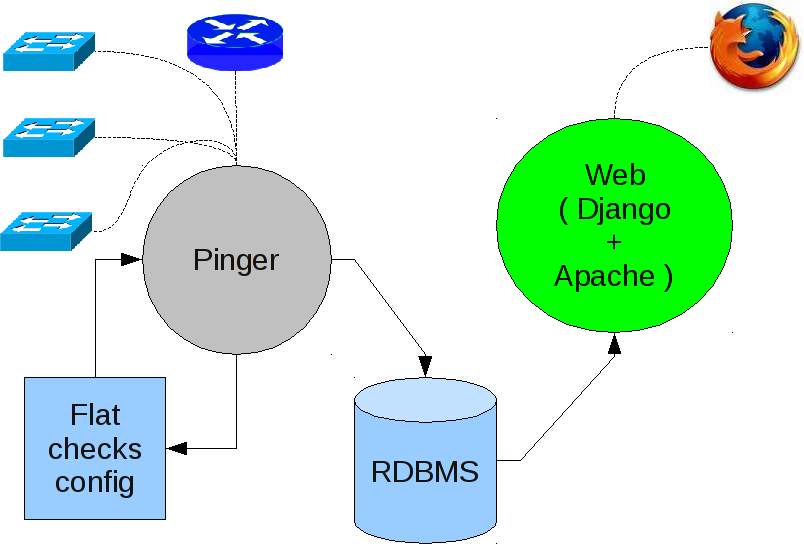
\includegraphics{DjangoAndPinger.png}}
\caption{RDBMS + Web (legge conf e stato) + Pinger (legge conf, scrive conf e stato)}\end{figure}


\section{Fase 2: CLI e mappe}

Il risultato raggiunto nella rappresentazione dell'attività di monitoraggio non era nemmeno paragonabile
alla versione precedente, quindi le priorità stringenti erano soddisfatte.

A questo punto il lavoro è proseguito da un lato con il potenziamento dell'interfaccia web e quindi:
\begin{itemize}
\item {} 
le mappe topologiche delle reti (a cui è dedicata una sezione separata)

\item {} 
interazione minimale: ricerca e gestione di appunti, note temporanee

\end{itemize}

dall'altro con \textbf{l'implementazione della {}`Command Line Interface{}` (CLI)}.

Con la CLI è stata colta l'occasione per potenziare l'espressività della tassonomia dei controlli
definibili nel sistema e implementare un'interfaccia per l'operatore di rete esperto: non a caso
l'interprete dei comandi implementato è simile a quello del sistema operativo Cisco IOS
molto diffuso e apprezzato fra gli esperti di reti.

La CLI è realizzata interamente in Python e si appoggia allo stesso modello di dati
costruito per la parte web. Ciò è stato un notevole pregio nell'aver scelto una soluzione come Django
che implementa in modo chiaro la separazione delle componenti; oltre ovviamente al beneficio
di utilizzare software libero che ci ha consentito di copiare le funzioni di inizializzazione di Django
e riportarle nella procedura di inizializzazione della CLI.

L'interprete dei comandi è sviluppato in modo molto semplice e pratico. Anche qui si nota, come nel vecchio \emph{pinger},
l'approccio sistemistico fatto di funzioni piuttosto che di classi ed ereditarietà, di variabili globali invece
di attributi statici di classe, o ancor meglio di passaggi per riferimento.

Anche l'output della CLI viene prodotto su misura e in un primo momento non si pensa alla possibilità di astrarre
il backend di output in modo da poter inizializzare lo stesso codice su backend testuale, ncurses, o grafico piuttosto che di socket di rete.

Per fortuna successivamente, appena possibile, non è stato troppo impegnativo l'intervento degli sviluppatori
per aprire questo spiraglio nella rappresentazione dei dati,
mentre purtroppo per le variabili globali o la strutturazione del codice ci si è dovuti accontentare
dell'implementazione realizzata e che comunque, a onor del vero, funziona.

Con la CLI viene implementata nel database tutta la parte di configurazione di SANET (categorie, attributi, istanze)
e quindi ristrutturato il vecchio sistema di \emph{template} e definizione dei controlli.

La compatibilità è rotta, anche se la logica di fondo rimane simile.

I sistemisti al lavoro nelle installazioni in produzione di SANET
si trovano disorientati e rallenta di molto il processo di aggiornamento delle installazioni da quella che era
la versione 1.4 alla versione 2.0 (poi diventate 0.1.4 e 0.2.0 con il rilascio alla comunità open source).

In questa fase viene sottovalutato l'impatto di un tale aggiornamento e senza che nessuno se ne accorga,
si interrompe il dialogo fra i sistemisti e gli sviluppatori,
facendo sì che solo dopo alcuni mesi ci si accorga del mancato avanzamento delle installazioni in produzione.

In ogni caso, è stato raggiunto un altro importante obiettivo: il potenziamento della tassonomia dei controlli.
Ora si possono definire molti più controlli con meno sforzo.

\emph{Pinger} è stato adattato per leggere la nuova configurazione dal database e continua la sua attività come strumento di monitoraggio e quindi di aggiornamento dello stato.

La configurazione e la rappresentazione sono in mano a SANET. Notare che non viene provvisto, e ad oggi non è ancora implementato, un modo per configurare via web i parametri dei controlli: ciò è dovuto alla consapevolezza delle complesse realtà di rete gestite dall'azienda che non si possono normalizzare con l'esposizione di interfacce cosiddette \emph{user-friendly}.
\hypertarget{dev-second-architecture}{}\begin{figure}[htbp]
\centering

\scalebox{0.700000}{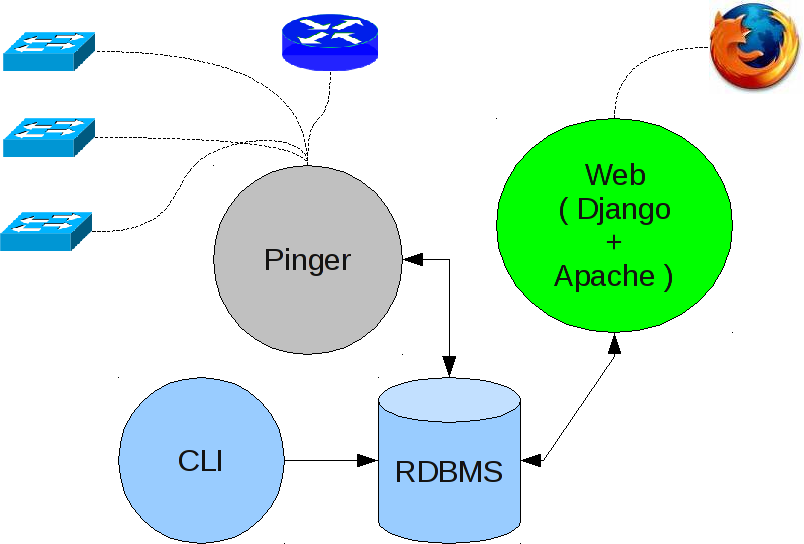
\includegraphics{DjangoAndPingerAndCLI.png}}
\caption{RDBMS + Web (legge conf e stato, scrive note e mappe) + CLI (scrive conf su RDBMS) + Pinger (legge conf e scrive stato su RDBMS)}\end{figure}


\section{Fase 3: Poller}

Entra un nuovo sviluppatore nella squadra. \textbf{Obiettivo riscrivere {}`pinger{}` in Python} e con questo:
\begin{itemize}
\item {} 
decurtare le ultime rimanenze di \emph{pinger}

\item {} 
aumentare l'espressività del linguaggio per la definizione delle espressioni con cui verificare lo stato ed effettuare le misurazioni

\item {} 
avere un sistema più scalabile grazie al \emph{multithread}

\end{itemize}

Se prima ci si era occupati dei meccanismi di ereditarietà fra i controlli e le categorie, ora ci si concentra sulla singola espressione da verificare. Si realizza un linguaggio con una propria grammatica, dotato di contesto e operatori con tipizzazione dinamica degli operandi. Questa nuova implementazione consente di esprimere ulteriori tipi di controlli; vegnono implementate:
\begin{itemize}
\item {} 
funzioni di adiacenza \emph{bgp} ed \emph{ospf}

\item {} 
controlli su \emph{ntp}

\item {} 
interrogazione \emph{WMI} tramite \emph{wmic} per i \emph{server Windows}

\item {} 
esecuzione comandi esterni (e quindi integrazione \emph{ZenPacks}, \emph{JMX} o \emph{plugins Nagios})

\item {} 
\emph{wildcards} per \emph{OID SNMP}

\item {} 
operatori di \emph{match} sottostringa

\end{itemize}

oltre al meccanismo di \emph{escalation} che consente di ridurre al minimo il rumore per gli allarmi ``a cascata''.

Anche in questo caso si può sfruttare il modello di dati già usato dalla CLI e dallo application server
e, vista l'elevata occupazione di memoria e la frequenza di operazioni di \emph{update} nel database,
si implementano meccanismi ad-hoc che sono più performanti di quelli offerti dal Django stesso.

Non mancano i \emph{bug} nella libreria NetSNMP e nel suo \emph{binding} Python: vengono segnalati, uno minore viene risolto,
per il resto si trovano \emph{workaround}.

Frattanto prosegue lo sviluppo delle mappe e il lavoro di promozione presso i clienti dell'azienda.

La realizzazione del \emph{poller} è la svolta finale che consente al gruppo di procedere verso il rilascio.
Ora il vecchio \emph{pinger} è completamente sradicato e SANET lo sostituisce completamente superandone i limiti.

Un ulteriore miglioramento per la fruibilità dei dati è costituito dalla segnalazione degli allarmi tramite \emph{feed RSS},
o dal recupero degli stessi tramite una semplice interfaccia \emph{XML-RPC} che ricorda l'operazione \emph{snmpwalk}.
\hypertarget{dev-architecture}{}\begin{figure}[htbp]
\centering

\scalebox{0.700000}{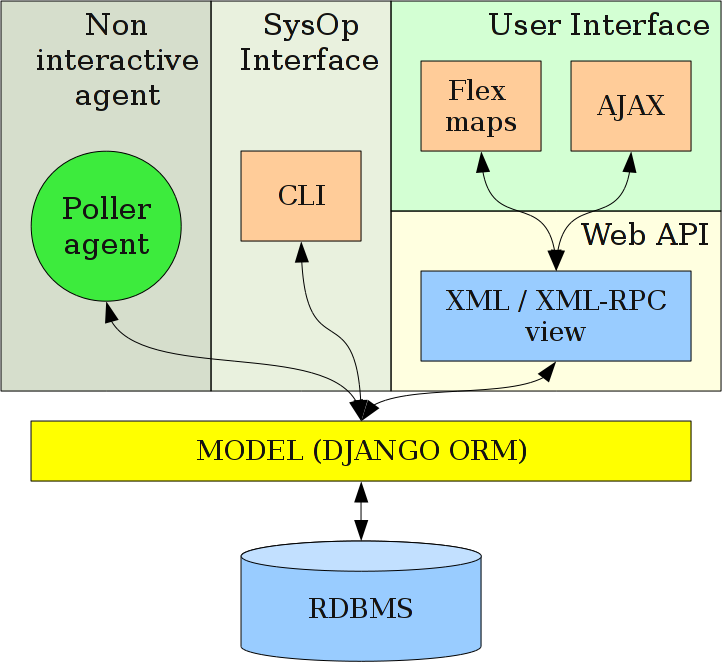
\includegraphics{Architettura.png}}
\caption{Architettura completa di SANET (RDBMS + Web + CLI + Poller)}\end{figure}


\section{L'impulso del Master FOSSET0809}

Durante questo ultimo anno ho avuto modo di frequentare il Master FOSSET
su proposta e con il sovvenzionamento dell'azienda.

Ritengo opportuno dedicare una breve sezione all'influenza che questa attività
di formazione ha avuto sul processo di sviluppo di SANET.

Un apporto importante si è verificato nella filiera di sviluppo di
tutto il software aziendale grazie al corso di \emph{Strumenti di sviluppo collaborativo}
e in particolare:
\begin{itemize}
\item {} 
uso degli \emph{hooks} per i sistemi di versionamento

\item {} 
strumenti di \emph{literate programming}

\end{itemize}

In questo modo abbiamo potuto realizzare l'infrastruttura di sviluppo presentata
in figura \hyperlink{dev-infrastructure}{\emph{Schema dell'infrastruttura di sviluppo}}.
\hypertarget{dev-infrastructure}{}\begin{figure}[htbp]
\centering

\scalebox{0.700000}{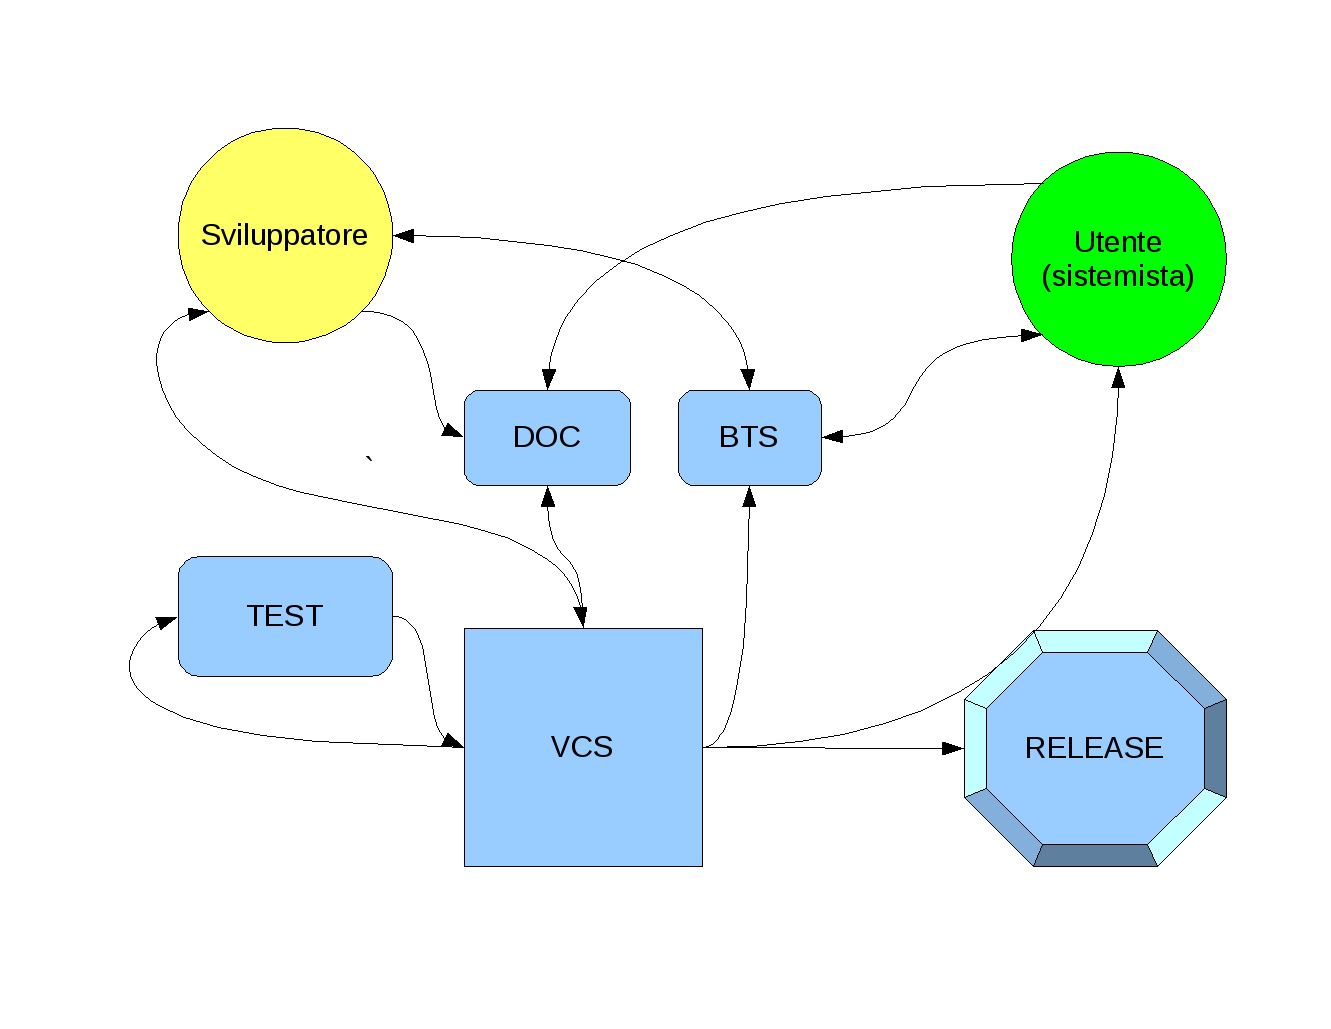
\includegraphics{InfrastrutturaDiSviluppo.png}}
\caption{Schema dell'infrastruttura di sviluppo}\end{figure}

Per quello che riguarda il corso di \emph{Project management} invece, abbiamo cercato di mantenere,
man mano che il team si allargava (con l'arrivo del nuovo sviluppatore) un approccio \emph{Agile} alla risoluzione
dei problemi, anche se non c'erano risorse per provare un vero e proprio \emph{Scrum} come avrei voluto.

Altri tentativi di adozione sono stati:
\begin{itemize}
\item {} 
la tecnica del pomodoro

\item {} 
\emph{test driven development}

\end{itemize}

entrambi interessanti, ma purtroppo naufragati a causa del piccolo team autogestito
e dal fatto che la crescita deve procedere per gradi.

Alcune sperimentazioni e introduzioni importanti sono derivate dai progetti:
\begin{itemize}
\item {} 
\textbf{Django history} realizzato per \emph{Fondamenti di sistemi liberi} ci ha consentito di sperimentare
un meccanismo versatile ed efficace per mantenere con Django
uno storico temporale di alcune tabelle del database. L'implementazione realizzata supera alcuni
dei limiti rilevati dall'autore Marty Alchin che purtroppo non ha più risposto ai miei messaggi.
In ogni caso il modulo realizzato può essere tranquillamente integrato così come è in SANET
per la gestione del log dei cambi di stato.

\item {} 
\textbf{Syslog collector} per il corso di \emph{Reti} è stato rilasciato come ulteriore prodotto LABS su
\href{http://syslog-agentx.sourceforge.net/}{http://syslog-agentx.sourceforge.net/} .
Esso consente a SANET (e non solo) di implementare una serie innumerevole di nuovi controlli
dato che esporta via SNMP informazioni su match di espressioni regolari in messaggi di \emph{syslog}.

\end{itemize}
\begin{figure}[htbp]
\centering

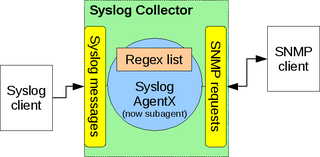
\includegraphics{SyslogCollector.png}
\caption{Syslog collector}\end{figure}
\begin{itemize}
\item {} 
Il lavoro effettuato per il supporto ai \emph{prepared statement} in Django con \emph{backend} PostgreSQL per il
corso di \emph{Basi di dati e applicazioni web} è servito per capire che non avremmo avuto un aumento
di prestazioni significativo con l'introduzione in SANET degli \emph{statement} precompilati.

\end{itemize}

\resetcurrentobjects
\hypertarget{--doc-networkmaps}{}

\chapter{Uno sforzo importante: le mappe}

Dedichiamo un capitolo all'implementazione ed evoluzione delle mappe di rete di SANET,
dato che proprio questa evoluzione è parte consistente del project work rilasciato insieme con questo documento.

Dopo la rappresentazione dell'attività di monitoraggio in un'interfaccia web 2.0 si è deciso di implementare
subito la visualizzazione delle mappe di rete per i contenitori.


\section{La scelta fra SVG o Flash}

La decisione di realizzare mappe interattive della rete ci ha subito posti
davanti alla scelta fra le tecnologie grafiche per il web: SVG o Flash.

In passato (v. \hyperlink{first-attempt-failed}{\emph{Un primo tentativo fallito}})
era stata implementata una versione basata su \emph{Scalable Vector Graphic} (SVG) in modo da ottenere
un risultato più aperto rispetto all'alternativa Flash di Macromedia ora Adobe.

Da quello che è stata la nostra esperienza, SVG risulta essere lento, e,
paradossalmente, anche se è uno standard \emph{più aperto} di Flash, Flash risulta essere più
diffuso fra le varie piattaforme e, purtroppo, la compatibilità con Internet Explorer è un fattore
critico in questi casi.

Inoltre, se da un lato lo standard SVG è comodo in quanto XML puro scrivibile comodamente anche tramite
il sistema di template messo a disposizione da Django, dall'altro
abbiamo molti esempi di applicazioni web che usano Flash,
ma non abbiamo praticamente alcun caso reale in cui si usi SVG.

Per dettagli ulteriori sulla valutazione fatta si veda l'appendice \hyperlink{svg-or-flash}{\emph{Appendice C - SVG o FLASH ?}}.

Nel frattempo Adobe ha rilasciato il \emph{framework Flex} con licenza Open Source,
il che ci avrebbe consentito di implementare applicazioni in Flash senza acquistare
licenze per costosi ambienti di sviluppo e
anche di poter apportare modifiche a librerie secondo le esigenze del caso.

Considerata quindi anche la possibilità di mantere \emph{vim}, il nostro IDE preferito,
si passa a Flash o più precisamente a Flex.


\section{La topologia della rete}

Per rappresentare la topologia della rete si è deciso di partire dalla libreria \emph{SpringGraph} di Mark Sheperd.

A questo punto è necessaria una premessa per capire la filosofia di SANET:
con SANET si desidera vedere tutto e solo quello che si intende monitorare,
quindi non solo si fa a meno dell'\emph{autodiscovery} dei collegamenti di rete,
ma anche degli algoritmi di posizionamento automatico dei nodi sulla mappa. Entrambe le attività
vengono affidate al sistemista di turno che ha il compito di configurare l'installazione specifica.

Per il posizionamento predefinito dei nodi di rete e dei contenitori
si è usato, e si usa ancora oggi, \emph{graphviz}.
Le posizioni sono poi modificabili dai soliti sistemisti, o anche dall'utente tramite interfaccia grafica.

L'evoluzione interessante, che costituisce parte corposa in questo project work, si è verificata tra la prima
e la seconda implementazione delle mappe di rete: vediamo ora quali erano caratteristiche e limiti della prima
versione e come sono stati superati.

Inizialmente era stato creato uno strato superiore alla libreria che:
\begin{itemize}
\item {} 
non usasse gli algoritmi di posizionamento automatico

\item {} 
posizionasse i vertici del grafo secondo le posizioni passate dal server

\item {} 
rappresentasse risorse differenti: nodi e contenitori in questa fase sono entrambi vertici della mappa

\item {} 
aggiornasse periodicamente lo stato degli elementi rappresentati: dei nodi, dei contenitori e dei collegamenti.
Lo stato dei collegamenti poteva (e può ancor oggi) essere rapprentato anche da un gradiente (trattasi di una
situazione temporanea o di un errore di configurazione),
in cui le verifiche effettuate sulle estremità del link restituiscano uno stato differente.

\end{itemize}

Nella prima implementazione, quella del rilascio alla CONFSL09, ogni contenitore
aveva associata un'unica mappa in cui venivano visualizzate le risorse direttamente incluse
e i collegamenti fra esse.

Nelle figure \hyperlink{map-generic}{\emph{Mappa prima versione: collegamenti fra i contenitori (notare i blu)}} e \hyperlink{map-core}{\emph{Mappa prima versione: icone personalizzate}} riportiamo alcuni esempi di mappe della prima implementazione.
\hypertarget{map-generic}{}\begin{figure}[htbp]
\centering

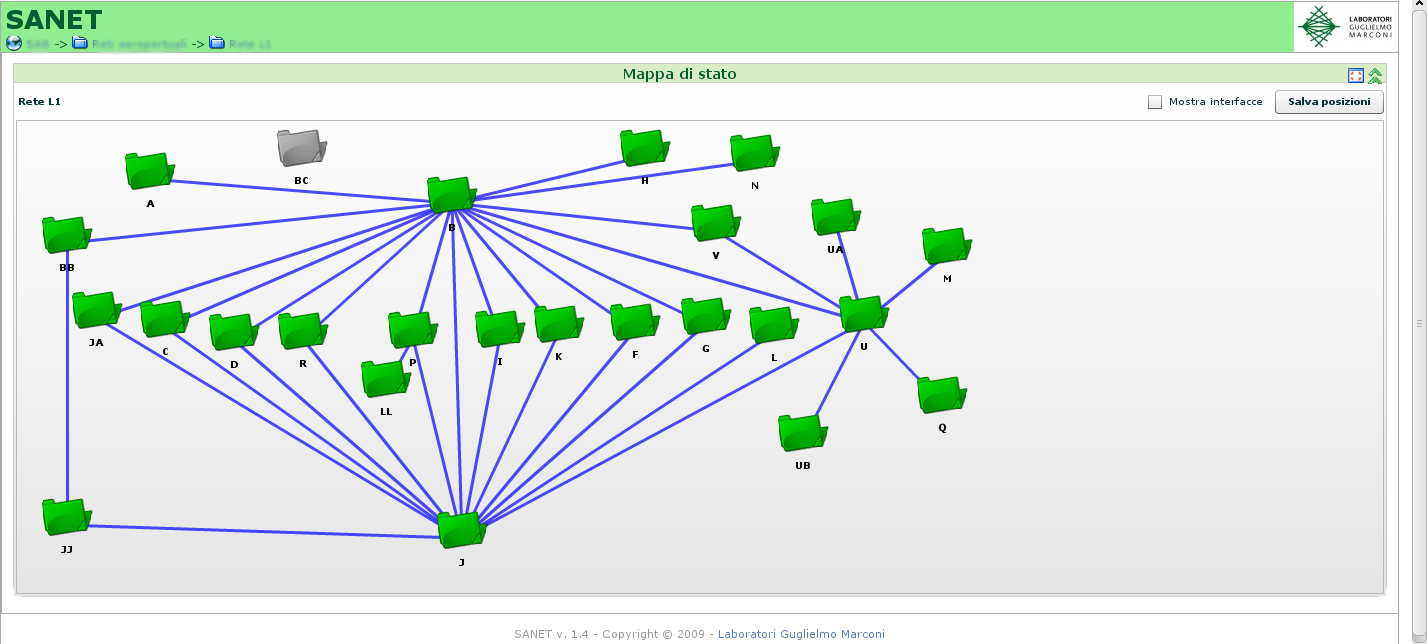
\includegraphics{mappa-generica-schermo-intero.png}
\caption{Mappa prima versione: collegamenti fra i contenitori (notare i blu)}\end{figure}
\hypertarget{map-core}{}\begin{figure}[htbp]
\centering

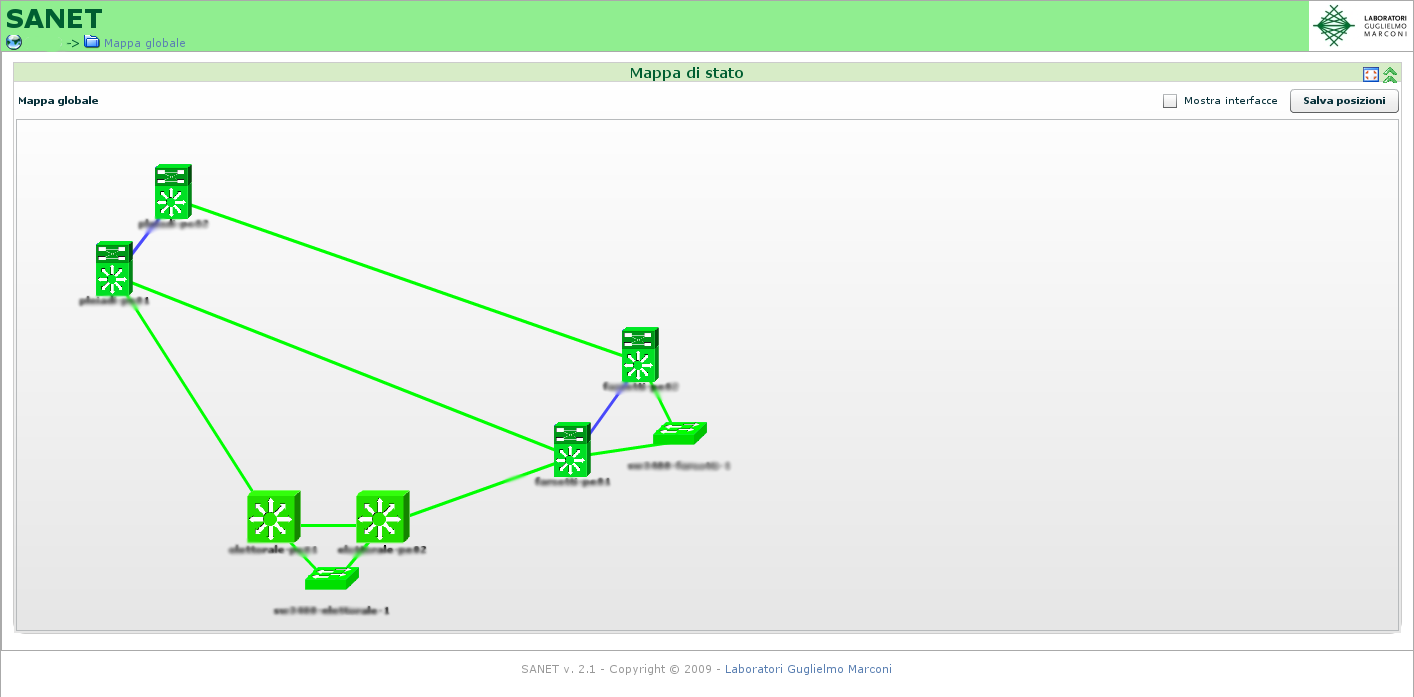
\includegraphics{mappa-core.png}
\caption{Mappa prima versione: icone personalizzate}\end{figure}

Nella nuova versione abbiamo voluto introdurre le seguenti funzionalità:
\begin{itemize}
\item {} 
rappresentare contenitori aperti e risorse contenute (clustering)

\item {} 
rappresentare mappe dei contenitori adiacenti al contenitore selezionato

\item {} 
visualizzare le singole interfacce di rete e il loro stato

\item {} 
superare il limite del grafo semplice che non consentiva di visualizzare link multipli fra gli stessi due vertici
(in caso di apparati con collegamenti ridondati o di contenitori con più apparati interconnessi veniva mostrato un arco blu)

\item {} 
rappresentare differenti parametri: alternativamente alla rappresentazione dello stato,
visualizzare il carico della rete o i valori relativi al protocollo Spanning Tree fra gli switch

\item {} 
aprire e chiudere contenitori da interfaccia utente

\end{itemize}


\subsection{La seconda implementazione}

Per superare i limiti elencati si è inizialmente provata la libreria \href{http://code.google.com/p/birdeye/}{RaVis}
che è più avanzata rispetto a \emph{SpingGraph}, ma purtroppo le esigenze di personalizzazione,
con particolare riguardo al \emph{clustering}, hanno fatto sì che tornassimo ad utilizzare
la soluzione precedente già conosciuta.

Quindi, seppur basandoci sulla stessa libreria,
siamo ripartiti con una riscrittura totale dell'implementazione precedente,
integrando ovviamente di volta in volta alcune parti che ritenevamo congrue alle nuove esigenze.


\subsubsection{Lato server}

Innanzi tutto è stata ristrutturata la parte server.

È stata creata una nuova applicazione Django denominata \emph{map} che si appoggia ad
un modello di dati ibrido: da una parte esso include le classi \emph{MapEnv} e \emph{MapOpenContainer}
che si appoggiano a tabelle nel database, dall'altra le
classi \emph{MapRoot}, \emph{OpenContainer}, \emph{OpenNode}, \emph{ClosedContainer}, \emph{ClosedNode}, \emph{ClosedIface}, \emph{MapEdge} che non
hanno un corrispettivo nel database, ma fungono da classi \emph{proxy} per gli oggetti di SANET e i corrispondenti \emph{dot} di \emph{graphviz}.

\emph{MapEnv} contiene la lista delle mappe disponibili nel sistema con gli attributi relativi.

Essa ha 2 campi fondamentali:
\begin{itemize}
\item {} 
\emph{bound\_container}: una chiave esterna che identifica a quale contenitore è associata la mappa,
ossia relativamente a quale contenitore deve essere visualizzata. Possono esistere più mappe associate
allo stesso contenitore. Per soddisfare l'esigenza di rappresentazione di mappe di adiacenza si è
pensato di introdurre la possibilità di associare mappe arbitrarie ad ogni contenitore

\item {} 
\emph{open\_containers}: che è un campo molti-a-molti attraverso il quale ogni mappa identifica i contenitori
aperti da rappresentare. Le risorse visualizzate nella mappa saranno tutte quelle direttamente incluse
nei contenitori aperti oggetto di questa relazione.
In questo caso la tabella referenziata è proprio quella della classe \emph{MapOpenContainer} che pertanto non ha bisogno di descrizione:
il suo scopo è infatti di rappresentare la relazione molti-a-molti che esiste fra \emph{MapEnv} e \emph{Container}.

\end{itemize}

Di seguito il semplice schema E-R dell'applicazione \emph{map}.
\begin{figure}[htbp]
\centering

\scalebox{0.700000}{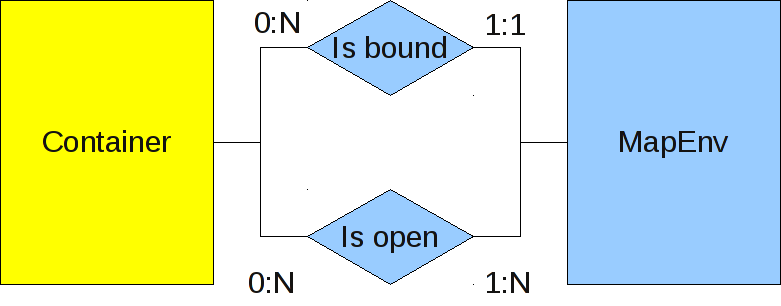
\includegraphics{map-ER.png}}
\caption{Schema E-R per le mappe}\end{figure}

Come dicevamo
\emph{MapRoot}, \emph{OpenContainer}, \emph{OpenNode}, \emph{ClosedContainer}, \emph{ClosedNode}, \emph{ClosedIface}, \emph{MapEdge} non
si appoggiano al database, ma fungono da classi \emph{proxy} verso due tipi di oggetti: una risorsa di SANET (contenitore, nodo, interfaccia) e il corrispondente oggetto \emph{pydot} che è il binding python per il \emph{dot} di \emph{graphviz}.

\emph{MapRoot} rappresenta la radice della mappa e fa da \emph{proxy} rispetto agli oggetti di classe \emph{MapEnv} e \emph{pydot.Dot}.
Ottiene le informazioni dall'istanza \emph{MapEnv} e procede ad istanziare gli altri oggetti di classi derivate da \emph{BaseDot} (che sarebbero poi gli \emph{Open*} e \emph{Closed*}). Infine processa tutti i link delle interfacce istanziate nella mappa e istanzia gli oggetti di classe \emph{Edge}. \emph{MapRoot} fa anche qualcosa di più: crea un container radice virtuale per ogni mappa in modo da avere coerenza anche in caso di contenitori aperti appartenenti a due gerarchie di contenitori differenti. In questo modo la rappresentazione di mappe arbitrarie è ricondotta al medesimo problema di rappresentazione della mappa di un singolo contenitore con possibilità di contenitori aperti innestati.

Le classi \emph{Open*} e \emph{Closed*} derivano da una classe comune \emph{BaseDot} che ha il compito di isolare proprio la logica
di \emph{proxy} verso le risorse di SANET e di \emph{pydot}.

Istanziando un oggetto di classe \emph{Open} si avrà a che fare con una risorsa di SANET e un'istanza di \emph{pydot.Cluster}. Mentre istanziando un oggetto di classe \emph{Closed} si avrà a che fare con una risorsa di SANET e un'istanza di \emph{pydot.Node}. Ciò significa che è stata completamente scorporata la natura intrinseca della risorsa di SANET dalla sua rappresentazione: se si vuole aprire un contenitore si passerà da un oggetto \emph{ClosedContainer} a un oggetto \emph{OpenContainer} che avrà fra i suoi attributi la medesima risorsa di class \emph{Container}.

Allo stesso modo per i nodi: se si desidera esplodere un nodo, ossia visualizzare tutte le interfacce all'interno in modo dettagliato per poter, in futuro, spostare il cavo UTP o la fibra da un'interfaccia a un'altra, è possibile farlo passando semplicemente da un \emph{ClosedNode} a un \emph{OpenNode}.

\emph{MapEdge} è una classe che include un oggetto \emph{pydot.Edge} più un'interfaccia sorgente e una destinazione.

Le mappe attuali utilizzano:
\begin{itemize}
\item {} 
\emph{OpenContainer} per rappresentare i contenainer aperti

\item {} 
\emph{ClosedContainer} per rappresentare i container chiusi

\item {} 
\emph{ClosedNode} per rappresentare i nodi

\item {} 
\emph{MapEdge} per gli archi

\end{itemize}

La gerarchia di \emph{MapRoot} viene serializzata in un documento XML.
La prima versione prevedeva solamente elementi di tipo:
\begin{itemize}
\item {} 
\textbf{\textless{}node\textgreater{}}: vertice del grafo, poteva essere un nodo o un contenitore

\item {} 
\textbf{\textless{}iface\textgreater{}}: elemento contenuto in \textbf{\textless{}node\textgreater{}} con la funzione di elencare solamente i nomi delle interfacce incluse nel nodo

\item {} 
\textbf{\textless{}edge\textgreater{}}: conteneva attributi per identificare gli endpoint di tipo \textless{}node\textgreater{} e gli endpoint di tipo \textless{}iface\textgreater{}

\end{itemize}

Nella nuova versione è stato introdotto il tipo \textbf{\textless{}subgraph\textgreater{}}  che altro non è che la serializzazione
di un'istanza di \emph{OpenContainer}. In questa versione è rilevante l'innestamento degli elementi XML
che stabiliscono in quale contenitore aperto si trovano gli oggetti rappresentati. Ciò è fondamentale
sotto 2 aspetti:
\begin{itemize}
\item {} 
il posizionamento di ogni elemento che deve essere calcolato relativamente al proprio contenitore aperto

\item {} 
lo spostamento di ogni elemento che deve considerare i limiti del proprio contenitore aperto.
Attualmente l'implementazione espande il contenitore aperto dell'elemento se esso viene spostato oltre il limite
del lato destro e del lato inferiore dello stesso.

\end{itemize}

In \hyperlink{map-xml}{\emph{Appendice D: XML prodotto per una mappa con contenitori aperti}} riportiamo un esempio di XML prodotto dalla nuova versione di SANET per rappresentare una mappa con contenitori aperti:

Una nota importante sulle interfacce di rete: è l'istanza \emph{ClosedNode} che serializza le interfacce
contenute nel nodo. Come vedremo le interfacce sono fondamentali per superare in modo apparente il limite del grafo semplice: purtroppo spesso non sono visualizzate e rendono più corposo lo XML prodotto.


\subsubsection{Lato Flex}

Quando si è andati ad intervenire sulla parte Flex,
abbiamo cercato di evitare qualunque modifica alla libreria SpringGraph originale,
per poter installare gli aggiornamenti (di minor version) e i bugfix in modo trasparente.

Ciò non è stato possibile a causa di alcune modifiche necessarie ad implementare i meccanismi
in oggetti derivati, quindi sono state effettuate alcune variazioni alle \emph{signature} delle funzioni
e degli attributi che in alcuni casi sono passati ad esempio da \emph{private} a \emph{protected}.
Queste personalizzazioni sono state segnalate all'autore che in un primo momento aveva risposto
dicendo che non era contrario alle modifiche, ma lui aveva risolto in precedenza in altri modi
e avrebbe comunque verificato la nostra patch. Da quel momento in poi non si è più ricevuta alcuna risposta.

Molti sforzi sono stati dedicati all'implementazione delle mappe lato Flex.
Flex è un framework molto potente, ma molto complesso.

Di seguito spieghiamo la logica che risiede dietro i file più significativi:
\begin{itemize}
\item {} 
\emph{SANETMap.mxml}: questo il file applicazione. Il main.
Contiene l'interfaccia grafica applicativa con i controller grafici e le funzioni (astratte) che servono a recuperare i valori desiderati (\textbf{valori di stato, spanning tree, carico di rete}). In questa nuova versione
sono stati introdotti 3 slider per: \textbf{zoom, curvatura degli archi e trasparenza dello sfondo dei contenitori aperti}.
È presente un \textbf{check selezionabile per la visualizzazione delle interfacce di rete e dei loro nomi}.
Infine un bottone per il \textbf{salvataggio permanente delle posizioni dei nodi}.

\item {} 
\emph{MapInfoProxy.as}: proxy del tipo di richiesta specifica. Tutti gli \emph{handler} di invio e ricezione si registrano in questa classe. Il controller
grafico che seleziona il tipo di valore da visualizzare attiva il canale specifico di richiesta/ricezione.

\item {} 
\emph{NetGraph.as}: struttura del grafo di cui poi VisualNetGraph.as conterrà la rappresentazione. Include il un metodo statico per costruire il grafo dai dati XML ricevuti.

\item {} 
\emph{VisualNetGraph.as}: rappresentazione grafica della mappa. Qui vengono innestati i contenitori aperti (a partire dal contenitore radice virtuale) e le risorse in essi incluse. Inoltre vengono ospitati gli archi che devono poter connettere risorse presenti anche in container aperti differenti e disattivato l'algoritmo automatico di posizionamento.

\item {} 
\emph{SANETEdge.as}: rappresentazione degli archi. Qui si gestisce la direzione e il gradiente. 2 trucchi sono stati usati per superare le limitazioni del grafo semplice: il primo riguarda la direzione e il secondo i link multipli. La direzione viene passata nell'elemento XML \textless{}edge\textgreater{} e viene ricalcolata proprio in questo file. Invece l'intuizione che sta dietro al superamento dei link multipli fra due vertici, consiste nella consapevolezza che le interfacce di rete odierne (\emph{wired}) se connesse, interconnettono sempre e solo 2 endopoint. In questo caso va benissimo il grafo semplice. Quindi nelle nuove mappe l'arco non è più costruito fra 2 nodi o 2 container chiusi, ma fra le interfacce che essi stessi contengono siano esse visibili o invisibili.

\item {} 
\emph{NestedItem.as}: implementa la logica dell'innestamento degli elementi XML spiegata sopra.

\item {} 
\emph{SANETViewFactory.as}: in fase di rendering, istanzia l'oggetto \emph{Visual*} specifico relativamente ai dati XML di un elemento di \emph{NetGraph.as} dato in input

\item {} 
\emph{VisualBaseNetGraphElement.mxml}: classe base per gli elementi della mappa. Definisce il canvas e gli handler per gli eventi nell'interazione con l'utente (mouseover, mouseout, doubleClick, ...)

\item {} 
\emph{VisualCloseContainer.as}: rappresentazione di contenitore chiuso. È usato anche per la rappresentazione dei nodi chiusi. Dal punto di vista dell'interfaccia sono icone che hanno un'etichetta, un url, stessi handler per la gestione di eventi e conoscenza delle interfacce di rete incluse (\emph{VisualIface.as})

\item {} 
\emph{VisualOpenContainer.as}: rappresentazione di container aperto. Un riquadro con posizionamento diverso dell'etichetta, bordi colorati con il proprio stato (derivante dalle risorse incluse nello stesso) e conoscenza degli oggetti in esso contenute (\emph{VisualOpenContainer.as}, \emph{VisualCloseContainer.as})

\item {} 
\emph{VisualIface.as}: rappresentazione grafica delle interfacce di rete. Esse sono cerchi posizionati al centro del proprio \emph{VisualCloseContainer.as}. Di esse non è possibile salvare le posizioni. È molto interessante poter visualizzare lo stato di una singola interfaccia di rete.

\end{itemize}

Purtroppo al momento della scrittura di questo documento manca l'implementazione lato server del recupero dei valori quali carico di rete e stato dello spanning tree e quindi, sebbene l'implementazione lato client sia praticamente pronta, tali parametri non possono essere rappresentati nella versione 0.4 di SANET.

\emph{SANETMap.swf} è il file compilato dell'applicazione Flash, occupa circa 400KB
ed è l'unico che viene scaricato dal browser (e messo in cache) per la visualizzazione delle mappe in SANET.

Un'ultima nota su come ancora una volta il software libero ci è stato di aiuto
e in particolare il modulo di terze parti Flex Thunderbolt
che consente di effettuare il log dei messaggi nell'estensione FireBug di Firefox
(estensione fondamentale per ogni sviluppatore web).


\subsubsection{Interazione fra Javascript e Flex}

A corredare il tutto non poteva mancare un modulo per interagire con le mappe direttamente da Javascript
e viceversa. Questo è il modulo Flex Ajax Bridge provvisto da Adobe stessa (file \emph{bridge/FABridge.as}) ed è
stato fondamentale per dare coerenza nel tooltip informativo delle risorse e nel menu contestuale.
\begin{figure}[htbp]
\centering

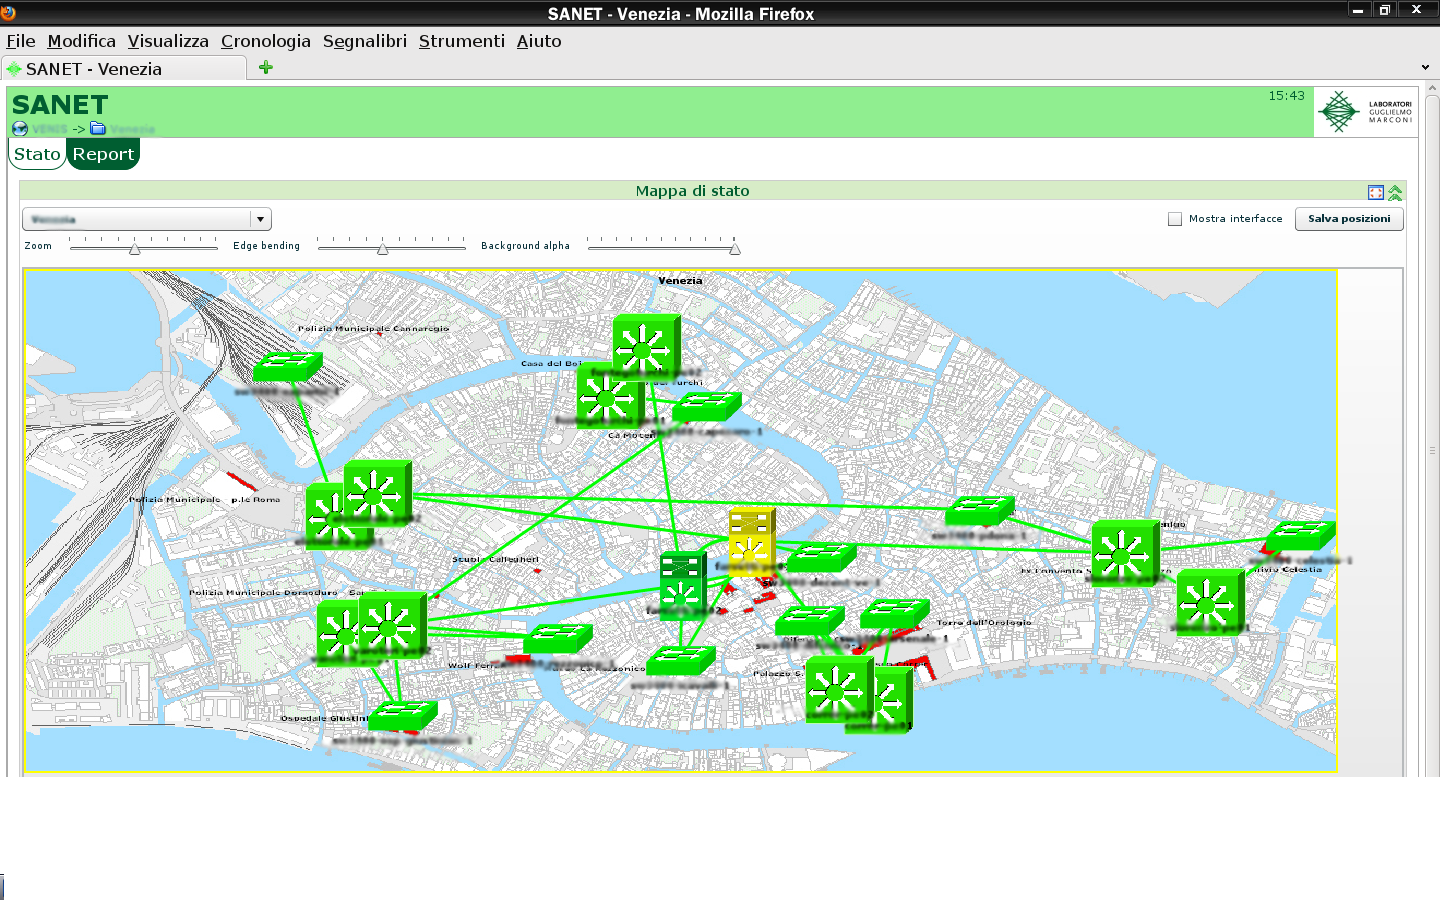
\includegraphics{map2-esempio-georeferenz.png}
\caption{Mappa con sfondo georeferenziato (precaricato)}\end{figure}
\begin{figure}[htbp]
\centering

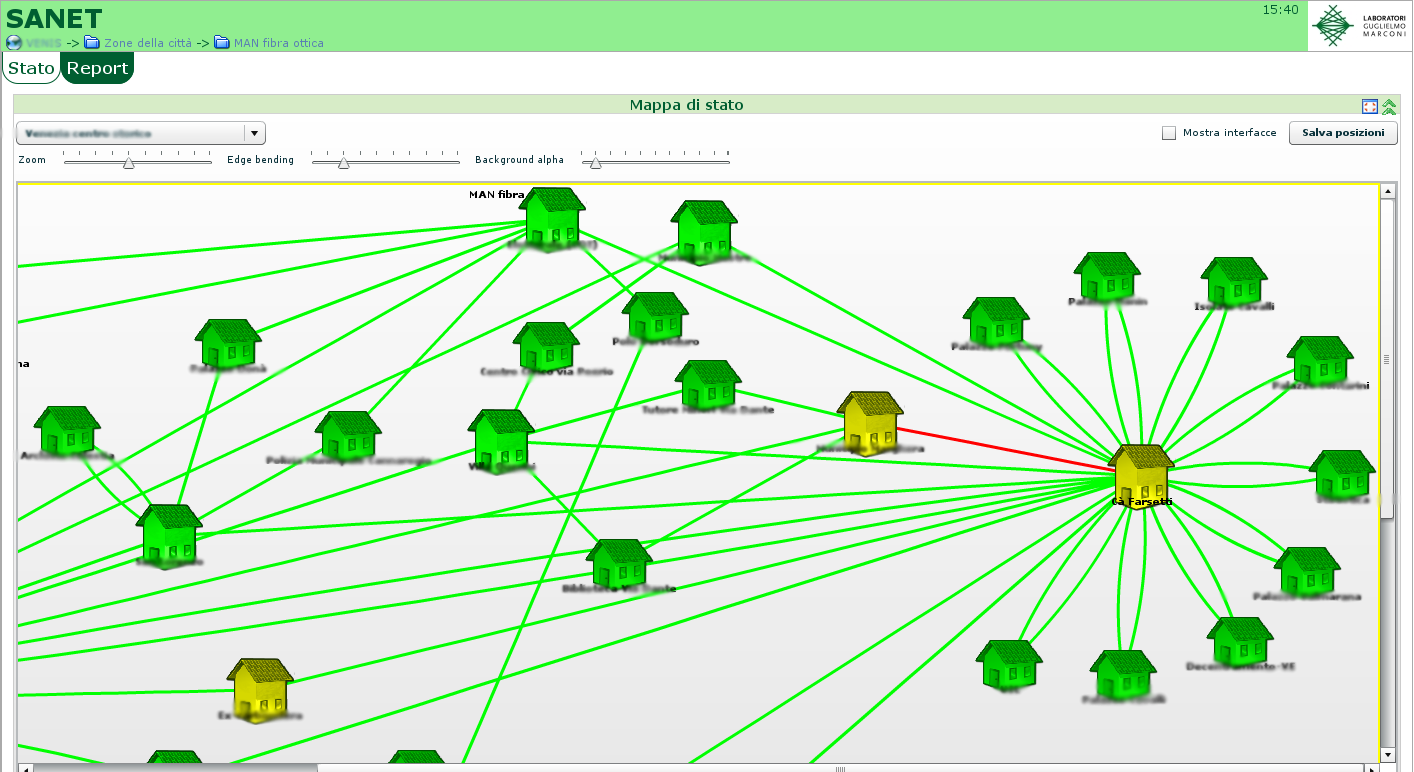
\includegraphics{map2-MAN-dettaglio.png}
\caption{Dettaglio di una MAN: notare gli archi doppi che partono dal grande edificio giallo a destra}\end{figure}
\begin{figure}[htbp]
\centering

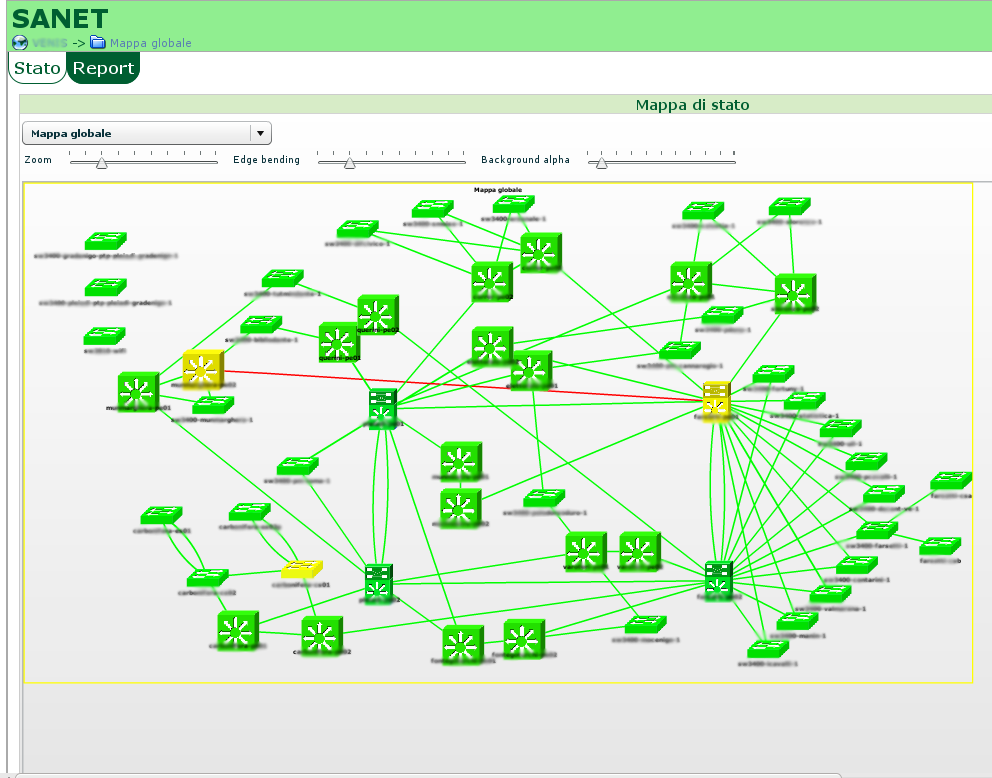
\includegraphics{map2-apparati.png}
\caption{Mappa di apparati: anche qui si notano archi doppi fra apparati ridondati}\end{figure}

\resetcurrentobjects
\hypertarget{--doc-release}{}

\chapter{Rilasciare SANET alla comunità}

Il processo di rilascio è una fase cruciale nella vita di un software libero.
È il momento in cui il software esce dalla sua nicchia ed entra a far parte della comunità.

Tecnicamente non si può dire che è il momento in cui il software libero nasce perché
un software è libero a prescindere dalla sua distribuzione, ma si può tranquillamente dire
che il rilascio è il momento in cui il software entra a far parte della comunità del software libero.

Per uno sviluppatore vuol dire mettersi in gioco, vuol dire trovare il tempo per spiegare
ed ascoltare. Per un'azienda vuol dire pubblicità, e vuol dire anche costi.

Un'azienda che non ha bisogno di pubblicità non è interessata a rilasciare il software.
Anche se un po' di pubblicità non guasta mai, bisogna considerare i costi ad essa collegata.

Rilasciare un software libero per un'azienda, significa porsi degli interrogativi e fare
delle scelte che altrimenti non avrebbe dovuto fare, significa un impegno a documentare adeguatamente
il software, significa creare dei canali di comunicazione con la comunità, significa
porre attenzione alle richieste della comunità.

Da tutto ciò quindi si deduce che non c'è solo un discorso di pubblicità, ma anche di qualità
del software e di apertura mentale di chi crede che il confronto sia in ogni caso costruttivo.

È per questo che secondo me bisogna credere nelle aziende che rilasciano i
propri prodotti e pongono attenzione alla comunità, mentre bisogna andare cauti con chi sostiene di
offrire soluzioni open source, ma che in realtà non giocano la propria parte secondo queste regole.


\section{Le scelte principali}

Riassumiamo le scelte fondamentali che LABS ha preso per essere pronta al rilascio di SANET:
\begin{itemize}
\item {} 
\textbf{Rilasciare tutto, o tenere un piccolo sottoinsieme di funzionalità ``separate''}:
non è raro trovare prodotti liberi di aziende che mantengono separate una serie di funzionalità
per la versione \emph{enterprise} con licenza meno aperta. Questo approccio può derivare da una serie di
considerazioni quali vantaggio competitivo, collaborazioni esterne, o il meno pulito di posizionare
i cosiddetti \emph{specchi per allodole}. LABS ha deciso di rilasciare tutto il software realizzato e anche
una corposa libreria di controlli. Questa è senza dubbio una scelta di grande apertura che sottolinea
la confidenza nel proprio operato e la consapevolezza che la ricchezza di un software simile consiste
soprattutto nel servizio di personalizzazione e assistenza h24 che si può offrire a strutture complesse
che necessitano di esperti sistemisti di rete... e la professionalità non si fa
con qualche riga di codice in più

\item {} 
\textbf{Quale licenza applicare}: dato che SANET è un'applicazione web, abbiamo optato per la AGPLv3.
L'intenzione è di evitare il \emph{problema Google}: un'azienda potente che inglobi SANET fornendo
un servizio di rete basato su di esso, ma senza essere obbligata a restituire il codice alla comunità
e tantomeno a noi

\item {} 
\textbf{Dove sviluppare il codice} o meglio dove gestire lo sviluppo del codice e la comunità degli utenti:
la risposta è stata \href{http://sanet.sourceforge.net}{Sourceforge.net}. Il portale di sviluppo software open source per definizione.
Sourceforge.net offre il sistema di versionamento Subversion (e ora anche GIT) e la recente possibilità di installare applicazioni esterne quali TRAC, MediaWiki o Wordpress, ci hanno convinto che sarebbe stata una scelta appropriata.
Infatti, in particolare grazie a TRAC, abbiamo potuto portare avanti il progetto senza cambiare il nostro modo di lavorare

\item {} 
\textbf{Quando uscire con la prima release}: una decisione non banale. Abbiamo deciso di uscire non appena
ci fossimo liberati totalmente del vecchio \emph{pinger}. In aiuto ci è venuta anche l'occasione della ConfSL09: un motivo in più per accellerare i lavori e rilasciare entro il 13 giugno 2009.

\end{itemize}


\section{Il primo rilascio alla ConfSL09}

\textbf{Sabato 13 giugno 2009 è il primo rilascio ufficiale di SANET}.

Momento storico per i LABS e in particolare per me che per qualche anno
avevo sviluppato software libero con il sogno, o l'ambizione di raggiungere questo obiettivo.

Cosa viene fatto per il rilascio di questa prima versione ?

Il minimo indispensabile:
\begin{itemize}
\item {} 
viene inserito un file LICENSE con la licenza AGPLv3

\item {} 
viene creato un tarball dell'ultima versione stabile

\item {} 
viene rilasciato il pdf dell'articolo per la CONFSL09 come guida base per l'utente

\item {} 
viene creata la home page del progetto: \href{http://sanet.sourceforge.net}{http://sanet.sourceforge.net}

\item {} 
viene attivato e impostato l'ambiente TRAC con le prossime milestone

\item {} 
viene creato e registrato il canale irc \#sanet nella rete freenode

\end{itemize}

La strada è tracciata. SANET è su Sourceforge.net.

Ora inizia un percorso: dalla cattedrale si va verso il bazaar.
Riportiamo a questo proposito la figura \hyperlink{from-tc-to-tb}{\emph{From the Cathedral to the Bazaar}} riferita allo studio
\emph{From the Cathedral to the Bazaar: An Empirical Study of the Lifecycle of Volunteer Community Projects}
di \emph{Andrea Capiluppi e Martin Michlmayr}.
\hypertarget{from-tc-to-tb}{}\begin{figure}[htbp]
\centering

\scalebox{0.800000}{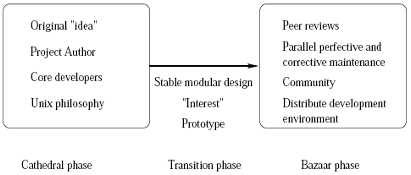
\includegraphics{DallaCattedraleAlBazaar.png}}
\caption{From the Cathedral to the Bazaar}\end{figure}

Nello studio i due autori spiegano come ogni progetto disseminato nel bazaar parta da una prima fase
caratterizzata dall'approccio a cattedrale.

Cosa c'è nella cattedrale ?
\begin{itemize}
\item {} 
Rappresentazione della rete
\begin{itemize}
\item {} 
Nodi

\item {} 
Interfacce

\item {} 
Controlli
\begin{itemize}
\item {} 
Target

\item {} 
Misure

\end{itemize}

\item {} 
Sito

\item {} 
Contenitori

\end{itemize}

\item {} 
Poller (agente di controllo)
\begin{itemize}
\item {} 
Legge la configurazione

\item {} 
Esegue i controlli

\item {} 
Agisce al verificarsi di determinate condizioni

\end{itemize}

\item {} 
Logica dei controlli
\begin{itemize}
\item {} 
Target UP

\item {} 
Target DOWN

\item {} 
Target FAILING

\item {} 
Target UNCHECKABLE

\item {} 
Target INACTIVE (trasparente)

\item {} 
2 limiti:
\begin{itemize}
\item {} 
Valore

\item {} 
Tolleranza temporale

\end{itemize}

\end{itemize}

\item {} 
Libreria dei controlli
\begin{itemize}
\item {} 
Nodo
\begin{itemize}
\item {} 
Raggiungibilità (MTU configurabile)

\item {} 
Occupazione CPU, FS, RAM, VMEM

\item {} 
Reboot

\item {} 
Presenza di un processo

\item {} 
Raggiungiblità TCP

\item {} 
Sincronizzazione con server NTP

\item {} 
Adiacenza BGP, OSPF

\item {} 
Match di un URL con una espressione regolare

\item {} 
WMI

\end{itemize}

\item {} 
Interfaccia (supporta variazione di ifIndex)
\begin{itemize}
\item {} 
Stato

\item {} 
Numero di errori

\item {} 
Pacchetti non unicast ricevuti

\item {} 
Full duplex

\item {} 
Traffico (supporta contatori a 32 e 64 bit)

\item {} 
STP

\item {} 
Variazione di stato

\item {} 
Variazione costo root bridge

\item {} 
Variazione porta root bridge

\end{itemize}

\end{itemize}

\item {} 
CLI per la configurazione
\begin{itemize}
\item {} 
Creazione e gestione di categorie di nodi, interfacce, controlli

\item {} 
Creazione e gestione di nodi, interfacce e controlli

\item {} 
Creazione e gestione di alberi e contenitori

\item {} 
Quando controllare

\item {} 
Quando e a chi mandare la segnalazione

\item {} 
Sospendere il controllo di un nodo

\item {} 
Snmpwalk integrato

\end{itemize}

\item {} 
Interfaccia web
\begin{itemize}
\item {} 
Visualizzazione dello stato e delle misure

\item {} 
Feed RSS

\item {} 
Mappe

\end{itemize}

\end{itemize}


\section{Andando verso il bazaar...}

Alla ConfSL09 il rilascio è stato annunciato come \emph{Open Source Prerelease}
a causa della mancanza di un'adeguata documentazione e dell'esternazione
del repository Subversion per lo sviluppo.

Ci siamo subito concentrati nel colmare queste lacune e quindi:
\begin{itemize}
\item {} 
la documentazione è stata completata e tradotta in inglese

\item {} 
abbiamo trasferito su Sourceforge tutto il repository Subversion con la storia dello sviluppo,
rimediando ad alcuni \emph{errori di giovinezza}: abbiamo eliminato alcune password che erano state
inserite in passato e la licenza è stata applicata in modo retroattivo

\item {} 
abbiamo riportato nel TRAC di Sourceforge i bug applicativi

\end{itemize}

Fatto il nuovo \emph{tarball} con i primi \emph{bugfix}, ci siamo anche confrontati internamente
sullo stato del software: quello che noi consideravamo versione 2.x
non poteva essere considerato alla stessa stregua dalla comunità del software libero.

Perciò abbiamo deciso di effettuare il \emph{downgrade} di versione dalla 2.3 alla 0.2.3:
SANET è funzionante, ma è ancora in evoluzione e soprattutto non ha ancora la \emph{confezione}
necessaria per essere almeno 1.0.


\section{Il secondo rilascio al termine del Master FOSSET0809}

Siamo a inizio novembre e SANET è andato molto avanti rispetto al rilascio di giugno.
C'è stato tutto il lavoro sulle mappe (fino ad agosto), ma non solo. Il \emph{poller} integra molti più controlli,
ed è stato realizzato un modulo per la reportistica.

In questo periodo la crescita della comunità non è stata fra le priorità LABS
che ha preferito spingere sulle nuove funzionalità.

A cinque mesi dal rilascio si contano:
\begin{itemize}
\item {} 
120 download dell'applicazione e 56 dell'articolo realizzato per la ConfSL09

\item {} 
un canale IRC frequentato solo da sistemisti LABS

\item {} 
un repository Subversion che è molto più avanti del tarball

\end{itemize}

Colgo l'occasione col dire che io, lo sviluppatore principale del progetto,
ho interrotto il rapporto di lavoro dipendente con i LABS il 30 settembre.
Questo aspetto è molto importante e darà adito ad alcune riflessioni che però lascio alla sezione
\hyperlink{retrospective-and-future}{\emph{Verifica e prospettive}}.

Di cosa ha bisogno SANET ora ?

Ho pensato di curare il rilascio di questa nuova versione, la 0.3.9.

I cambiamenti sono stati molti e ci avviciniamo alla 0.4.
È giunto il momento di realizzare la procedura di installazione che si occupi
di verificare se tutte le dipendenze del sistema sono soddisfatte.

È abbastanza frequente che si verifichino errori a causa di vecchie librerie,
o mancanza di alcuni prerequisiti.

L'evoluzione naturale del rilascio del software sarebbe di ampliare il bacino
di utenza e ampliare i canali di comunicazione con la comunità. Per fare questo
è innanzi tutto importante pacchettizzare il software per una distribuzione.
Un'altra idea sarebbe di aprire un blog specializzato.

Al momento, considerata l'evoluzione dei rapporti, non si è pensato di
proseguire riguardo a questi ultimi due passi. Si intende discuterne con LABS
che detiene il diritto di paternità del software e quindi l'interesse nella diffusione
dell'implementazione.

In questa fase abbiamo quindi congelato lo sviluppo e creato il file standard \href{http://docs.python.org/distutils/setupscript.html}{setup.py}
per la distribuzione di applicativi python. Lo script verifica le dipendenze
e installa il software. Inoltre è stato adottato \href{http://pip.openplans.org/}{pip} per la generazione
dell'elenco di librerie python richieste con le rispettive versioni.
Per quello che riguarda la verifica delle dipendenze fra applicativi i manutentori di moduli python
suggeriscono di occuparsene usando i gestori pacchetti delle distribuzioni specifiche.

Abbiamo cercato di andare oltre, per verificare le dipendenze rispetto ad applicativi
esterni. Sicuramente lo strumento per eccellenza a questo fine sono gli \emph{autotools}, ma
l'idea è giunta tardi e, alla data di stesura di questo documento, non c'è stato modo di provarli.
È stato invece realizzato lo script ad-hoc \emph{install\_requirements.sh} che verifica la presenza di corrette librerie
NET-SNMP e PostgreSQL che sono elementi cruciali del sistema.
La sua esecuzione è stata integrata nel \emph{setup.py} per mantenere comunque la procedura standard
di installazione pacchetti python.
Ripeto che il prossimo passo sarà ripassare gli \emph{autotools} e provare con quelli.

Il senso di creare la 0.3.9 (alpha 1) è quello di avere margine per alcune modifiche grafiche
nell'integrazione nell'interfaccia del modulo dei report che necessita di alcune migliorie prima della 0.4.

\resetcurrentobjects
\hypertarget{--doc-retrospectiveandfuture}{}

\hypertarget{retrospective-and-future}{}\chapter{Verifica e prospettive}

Indubbiamente SANET esiste, funziona e tecnicamente si può dire che è
uno degli strumenti più avanzati nel panorama dei Network Management System
Open Source.

Sicuramente può e deve ancora migliorare sotto l'aspetto della comunità,
delle performance, della distribuzione degli agenti, della personalizzazione
degli eventi.

Potrebbe anche interagire con sistemi di \emph{ticketing} per la gestione
del \emph{workflow} di risoluzione degli allarmi.

In questo capitolo si intende proporre una verifica
e analizzare alcuni possibili prospettive future
relativamente al processo di sviluppo e rilascio e agli attori
attualmente interessati al buon funzionamento e al miglioramento di SANET.


\section{Verifica}

Guardarsi alle spalle dopo qualche anno di lavoro non è semplice.
Neanche le dinamiche che hanno portato all'evoluzione di SANET sono semplici,
come non sono semplici le dinamiche della comunità Open Source.

Vivendo dall'interno questo processo ci si rende conto che alla fine
le uniche cose che contano veramente sono le priorità aziendali.
Chi è nel mondo dell'Open Source da anni non può non sapere che è questa
la regola che vale per i prodotti di successo. È il trionfo di un sano liberismo
in cui le priorità aziendali sono anche quelle che portano a un miglioramento sociale
e comunitario.

Purtroppo le priorità aziendali, accompagnate da un contesto sociale in cui la
mancanza di tempo e la fretta predominano, a volte portano a compiere scelte
affrettate e si perdono inevitabilmente occasioni di crescita derivanti da un confronto
più approfondito con lo stato dell'arte e la comunità del software libero.

Nel complesso io credo che la forte esperienza dei LABS nella gestione delle reti e il
precedente sistema di monitoraggio \emph{pinger}, abbiano giocato un ruolo fondamentale nella
decisione di non puntare ad integrarsi a soluzioni esistenti.
Questa scelta potrebbe essere criticata anche considerando che LABS storicamente non è un'azienda
di sviluppo software e quindi sarebbe stato più produttivo avvalersi della forza della comunità
invece che creare e mantenere un nuovo programma.
Allo stesso modo potrei dire che con una unità di sviluppatori più corposa si sarebbe potuto indagare meglio
sulle peculiarità degli altri sistemi di monitoraggio perché si sa ...
la barriera di entrata è più alta se si deve entrare in un progetto avviato.
Soprattutto se ci si deve entrare con un know-how importante da integrare.

Considerati questi aspetti, sebbene io stesso fossi promotore di un approccio più aperto
ed integrato con le soluzioni esistenti, comprendo le scelte che l'azienda ha fatto.

Ora che il prodotto è maturo per un uso interno, credo che sia il momento di aprirsi in modo
più deciso alla comunità. In questo modo ci si potrebbe avvalere anche di collaboratori esterni interessati allo sviluppo
di SANET che potrebbero apportare contributi in documentazione, codice, pubblicità o nuove idee senza gravare sui costi aziendali.

Riguardo alla tecnologia usata ritengo che siano state fatte scelte appropriate:
\begin{itemize}
\item {} 
Python è un linguaggio di programmazione versatile e veloce che consente programmazione funzionale, ad oggetti e a metaclassi

\item {} 
Django è un framework web che non snatura python e ne sfrutta ottimamente le potenzialità

\item {} 
PostgreSQL è potente e comunque la scelta di appoggiarsi ad un RDBMS è di indubbia utilità

\item {} 
Flash, per quanto riproducibile ottimamente solo con il plugin proprietario di Adobe è stupefacente

\item {} 
RRD è il punto di riferimento per le serie temporali e il consolidamento dei dati

\item {} 
RSS + XML-RPC e folksonomie sono tecnicismi del Web 2.0 che adattano SANET anche alla consultazione tramite strumenti esterni

\end{itemize}


\section{Prospettive}

Un altro punto su cui bisogna porre molta attenzione sono secondo me le prospettive che
si aprono a partire da uno strumento di software libero creato a cattedrale da un'azienda e poi rilasciato nella sua interezza.

Cosa succederà ?

Il rilascio sicuramente è ancora una scommessa, per l'azienda e per me che sono stato uno dei principali autori di SANET.
Date le logiche aziendali che hanno condotto fin qui il progetto,
non mi sembra che sia fra le priorità dell'azienda far crescere la comunità di sviluppatori intorno a SANET.

Ma il punto è un altro: SANET nasce come prodotto all'interno di LABS. Effettuando il rilascio alla comunità LABS,
pur non rinunciando al diritto (inalienabile) di paternità dell'opera, di fatto offre un ruolo centrale al prodotto
su cui convogliare l'interesse in modo diretto:
per accedere al programma, alla conoscenza e alle funzionalità da esso implementate non si deve più necessariamente
passare attraverso LABS.

È in questo, come si è ricordato più volte, che si denota una grande apertura di mentalità dell'azienda.

Ora, l'interesse è catalizzato dal prodotto e di fatto, ogni attore del mercato può \emph{dare una spinta} verso il miglioramento.

Ad esempio io in questo momento, nella scrittura di questo progetto finale di Master, sto scrivendo una documentazione
sull'evoluzione di SANET, e ho realizzato la procedura di installazione del software pur non essendo alle
dipendenze dell'azienda.

Poniamo caso che l'azienda \href{http://www.befair.it}{beFair} da me costituita nutra interesse per l'attività di monitoraggio delle reti,
o individui l'esigenza di un cliente che possa essere soddisfatta con degli aggiornamenti su SANET, ebbene, sarebbe interesse
dell'azienda beFair e dell'azienda LABS discutere del miglioramento ed integrarlo nella versione ufficiale di SANET.

Questo è il punto fondamentale e la grande apertura del rilascio alla comunità: siamo tutti curiosi di vedere
come si evolverà questa situazione.

\resetcurrentobjects
\hypertarget{--doc-appendix/oss-nms}{}

\chapter{Appendice A - Osservazioni su NMS open source in lista cisco-nsp}

La mailing-list \textbf{cisco-nsp} è una lista di discussione per persone che usano
apparati Cisco in Network Service Provider.

Riportiamo qui di seguito un messaggio che include, nella parte quotata, alcune osservazioni
sui sistemi di monitoraggio Open Source e la risposta dell'Ing. Michele Bergonzoni,
sistemista senior in reti di telecomunicazioni (nda: direi più un \emph{network god}), nonché
autore unico di \emph{pinger} e coautore di \emph{SANET}.

Il messaggio assume un significato di particolare importanza in quanto riesce a cogliere
gli aspetti tecnici più nascosti per cui si è deciso di sviluppare un sistema alternativo
per il monitoraggio delle reti.

Inizia qui il messaggio reperibile all'indirizzo
\href{https://puck.nether.net/pipermail/cisco-nsp/2009-July/062347.html}{{[}c-nsp{]} Free NMS Tools}:

\begin{Verbatim}[commandchars=@\[\]]
Michele Bergonzoni bergonz at labs.it
Fri Jul 17 09:26:28 EDT 2009

    * Previous message: @PYGZlb[]c-nsp@PYGZrb[] Free NMS Tools
    * Next message: @PYGZlb[]c-nsp@PYGZrb[] Free NMS Tools
    * Messages sorted by: @PYGZlb[] date @PYGZrb[] @PYGZlb[] thread @PYGZrb[] @PYGZlb[] subject @PYGZrb[] @PYGZlb[] author @PYGZrb[]

Saku Ytti @textless[]saku at ytti.fi@textgreater[] said:

@textgreater[] To me all OSS NMS solutions out seem like they are made by
@textgreater[] coder-in-server-admin not coder-in-network-admin, and as such seem to
@textgreater[]  have much more integration with servers than with network

This is one of the reasons why over the years we developed sanet, the
other being that many NMSs are very chatty and tend to keep you up all
night when relayed on pagers and SMS.

Sanet is OSS but in prerelease, meaning that we use it and it works, but
its documentation is not quite complete and it is not easy to install.
If you are willing to setup many python packages by hand and to explore
funcionalities without a concise HOWTO, or if you are just interested in
the OIDs, you can find it at sanet.sf.net, the SVN version being much
better (expecially for maps and reports) than the downloadable version.

We use it mainly in multivendor corporate networks, but we have one case
of cisco MPLS carrier network.

@textgreater[] Why don't they ship with MIBs or just specific OIDs for few top
@textgreater[] vendors important traps etc?

sanet has a a library of checks for common cisco, HP, fortigate and
other vendor's OIDs. Sorry we don't collect traps nor syslog in the
sanet DB, we usually transform traps to syslog (net-snmp snmptrapd) and
collect syslog (we are accustomed to grepping the results).

@textgreater[] Adding appropriate reaction classification.

Sanet does not react. You can trivially achieve that by binding scripts
to emails, etc., but we are quite scared of this kind of triggering and
we don't do it (yet).

@textgreater[] People want NMS to automatically monitor BGP

In the library there is the check for the BGP neighborship state:

"1.3.6.1.2.1.15.3.1.2.@$peer@_ip:@$community@PYGZat[]@$node == 6"

it is not "automatic" because in sanet you have to decide all the
monitoring that you want it to do.

@textgreater[] OSPF

We have the OSPF neighborship state check:

"1.3.6.1.2.1.14.10.1.6.byRegexpUnique(1.3.6.1.2.1.4.20.1.2,@textasciicircum[]@$ifindex@$).0:@$linked@_community@PYGZat[]@$linked@_node
== 8"

but it works only for point-to-point links. I'm sure we can make it better.

@textgreater[] IS-IS

Sorry no IS-IS here, but of course you can define your own if you know
the OIDs. Please contribute it back if you do.

@textgreater[] LDP

We have an LDP neighborship check:

"1.3.6.1.2.1.10.166.4.1.3.2.1.2.byBinaryIP(1.3.6.1.2.1.10.166.4.1.3.2.1.5:@$community@PYGZat[]@$node,@$peer@_ip):@$community@PYGZat[]@$node
== 2"

@textgreater[] status of some other CPU/memory than just control-plane

Well, for IOS we usually check processor memory and IO memory. OIDs and
suggestions are very, very welcome.

@textgreater[] Other thing that annoys me is how SNMP pollers are implemented,
@textgreater[] they're blocking

You are definitely right. Our poller is multithreaded but each thread is
blocking, with adjustable timeouts.

@textgreater[] While having SNMP poller poll 140k OID per second on 386 class PC is
@textgreater[] rather trivial, using two process strategy, where single process
@textgreater[] spews packets outs, and another listens what comes back, completely
@textgreater[] asynchronous

It was not so trivial for us, so we made it synchronous. The tricky part
is to collect all the SNMP vars used to form an expression in the same
moment (of course with some approximation), remembering what you asked
for at each poll cycle. It is trivial if you just check variables
against ranges, but we build complex expressions with current and past
variables.

Anyway, patches are welcome...

@textgreater[] I've also only seen alarms based on absolute values of different
@textgreater[] counters

sanet can combine current and past (last poll cycle) vars, like this
expression for a threshold on broadcast packets received:

"((1.3.6.1.2.1.2.2.1.12.@$ifindex:@$community@PYGZat[]@$node -
1.3.6.1.2.1.2.2.1.12.@$ifindex@#@$node) / @$delta) @textless[] @$threshold"

(@$delta is the time in second since last poll)

@textgreater[] This type of 'trending' module should be relatively easy, and could
@textgreater[] be reused by any counter values.

This is a good idea, I will try to think about how this can fit into our
existing software or if a new check type is needed for that.

@textgreater[] I demoed zenoss with 27 routers and it froze trying to poll their
@textgreater[] interface (granted there are very many interfaces)

We measure installations from the number of targets (yes/no checks) and
measures (graphs). One of our big ones is:

root at XXXXXX:@textasciitilde[]@# sanet-cli
Benvenuti in SANET 2 su XXXXX

sanet@# sh ver
...
Configuration defines 831 interfaces, 523 nodes, 409 links, 9868
targets, 2089 measures.
Targets summary: 9 down, 1 failing, 38 uncheckable, 0 out of time, 9820 up
Measures summary: 2042 updated in last 2 mins, 2089 in last 5 mins, 2089
in last 30 mins

(this is running on a XEN VM, I/O being the bottleneck)

I'm sure people on this list will appreciate the configuration via CLI
(web is used for displaying the status), which is shamelessly copied
from IOS. This was "sh ver", and in order to configure monitoring you
start with "conf t". You will probably appreciate physical maps (a /30
is a line, not a line with a cloud in between), NTP checks, IPv4/IPv6
pings with adjustable payload length, iface designation by name, MAC,
IP, CDP neighbor, route, IOS description, etc (no ifindex blues).

Hope this helps,
                                    Bergonz


--
Ing. Michele Bergonzoni - Laboratori Guglielmo Marconi S.p.a.
Phone:+39-051-4392826 Fax:+39-051-6153683 e-mail: bergonz at labs.it
alt.advanced.networks.design.configure.operate
\end{Verbatim}

\resetcurrentobjects
\hypertarget{--doc-appendix/security}{}

\chapter{Appendice B - Analisi della sicurezza di SANET}

In questa appendice si vuole effettuare una breve disamina delle problematiche di sicurezza di SANET.

SANET è un software Web il che vuol dire tutto e non vuol dire niente.
Diciamo che dialoga all'esterno tramite il protocollo HTTP.

Oltre ad ascoltare richieste HTTP, SANET effettua disparate richieste sulla rete da cui si aspetta
determinate risposte. Tali richieste vengono fatte molto spesso tramite protocollo SNMP,
ma è altrettanto possibile che siano implementati comandi ad-hoc per interagire con qualunque altro esotico servizio.

Infine SANET dispone della CLI di configurazione che è accessibile in locale
e per il quale si applica una politica di \emph{trust} degli utenti del sistema.

Quindi gli attacchi esterni possono provenire da:
\begin{itemize}
\item {} 
richieste malformate veicolate sulle porte HTTP

\item {} 
informazioni ricevute in risposta alle richieste effettuate per la rete monitorata

\end{itemize}

Mentre gli attacchi interni da:
\begin{itemize}
\item {} 
\emph{code injection} in comandi impartiti nella CLI locale

\item {} 
\emph{sql injection} nel database locale

\end{itemize}

oltre ai più classici \emph{Denial Of Service} per l'esterno e \emph{bug} di libreria di cui segnaleremo solo un caso critico.


\section{Attacchi esterni}

Iniziamo col dire che SANET soffre ancora di problemi di performance. È un sistema \emph{CPU-bound}
(oltre che \emph{Network-bound} per quello che riguarda il monitoraggio delle condizioni di rete), per cui non è difficile realizzare un attacco
Denial Of Service e fare in modo che altri utenti non possano accedere al sistema di monitoraggio e visualizzare
lo stato della rete.

Tolto il problema del Denial Of Service bisogna considerare il tipo di operazioni che vengono esposte via web:
\begin{itemize}
\item {} 
richiesta generica di un url

\item {} 
salvataggio note e posizioni degli elementi nella mappa: queste operazioni scrivono dati nello RDBMS

\end{itemize}

La richiesta generica di un url potrebbe dare problemi in caso di pacchetto HTTP malformato,
oppure di corpo della richiesta forgiato ad-hoc per operazioni di code injection.

SANET è basato su Django che nelle installazioni in produzione è gestito tramite l'handler \emph{mod\_python} di Apache.
Quindi per quello che riguarda i livelli ISO/OSI fino al livello HTTP , la sicurezza è garantita dall'implementazione
dello stack TCP/IP del sistema operativo di installazione (GNU/Linux per noi), mentre per il livello HTTP abbiamo Apache Web Server.

Il contenuto del pacchetto HTTP invece viene trasmesso a livello applicativo anche in questo caso molto robusto:
\begin{itemize}
\item {} 
del web server non occorre dire altro

\item {} 
Django dispone di un ottimo sistema di quoting e sanitizzazione dell'input grazie alla libreria cgi di Python

\item {} 
inoltre i parametri valorizzati compilando i \emph{form} nella canonica interfaccia web, vengono serializzati tramite la libreria \emph{Javascript Prototype} che ne garantisce il corretto quoting nell'url della richiesta in caso di una \emph{GET}, o nell'url e nel \emph{payload} in caso di una \emph{POST} (operazioni HTTP più comuni). Certo, questa è una considerazione esclusivamente marginale se si pensa che in un attacco informatico di solito l'input non viene fornito tramite l'interfaccia web applicativa.

\end{itemize}

Rimane la possibilità di iniezione di codice attraverso risposte malformate alle richieste di monitoraggio di \emph{poller}.
In questo caso le richieste SNMP sono state incapsulate e attualmente si appoggiano ai binding python di NetSNMP.
La nota positiva è che essendo incapsulati possono essere facilmente rimpiazzati da altri moduli che implementano richieste SNMP,
la nota negativa è che ogni tanto l'implementazione attuale raramente va in \emph{Segmentation fault}. Questo problema si è verificato
per siti molto grandi, dove incide molto la latenza della rete nell'effettuazione dei controlli.

Dopo una indagine approfondita del problema non se ne è riuscita ad individuarne la causa, e il problema (che io sappia)
non è stato sottoposto alla comunità di sviluppo per mancanza di informazioni sulla riproducibilità e la particolarità delle
reti in cui questo problema si verifica. È stato comunque realizzato un \emph{kludge} con un processo padre che ha il solo compito
di supervisionare l'esistenza del figlio che effettua i controlli di rete e riavviarlo in caso non esista più.

Gli altri controlli di rete sono implementati da funzioni apposite e il parsing dei risultati effettuato di volta in volta
a seconda del tipo di controllo configurato. In genere il valore di ritorno viene considerato come stringa o come uno specifico
tipo di dato dipendentemente dall'operatore definito nel controllo e relativamente a questo correttamente interpretato.
In ogni caso mai valutato.

Il sistema non riceve trap SNMP dagli apparati.

Non si può chiudere la sezione sugli attacchi esterni senza porre in evidenza il rischio relativo alla compromissione del DNS
cui \emph{poller} dirige numerose richieste. Se infatti venisse compromesso il DNS interrogato, si potrebbero indirizzare a piacimento
tutte queste richieste ad esempio ad un singolo host e generare un DoS. Questo considerato anche che in reti mediamente
complesse il processo dispone di circa 40 thread che fanno richieste in parallelo.


\section{Attacchi interni}

Come si accennava prima, è stata adottata una politica di sicurezza \emph{trust} per gli utenti del sistema locale,
quindi è ovvio che se qualcuno riuscisse ad entrare nel sistema con un account autorizzato, molto probabilmente
riuscirà a far fare a SANET quello che vorrà.

Ma l'altra domanda che ci si pone è se SANET possa o meno presentare un pericolo reale per il sistema,
o meglio, se sia possibile ottenere un accesso privilegiato sfruttando un problema di sicurezza di SANET.

Una prima considerazione da fare è che il \emph{poller} viene eseguito come utente \emph{root} del sistema,
perché deve poter forgiare pacchetti RAW per fare ICMP ECHO REQUEST (ping). Questo già potrebbe essere
facilmente migliorabile nel caso si avesse a disposizione un kernel Linux che supporti le \emph{capabilities}
e in particolare si potrebbe creare un account con la capability \emph{CAP\_NET\_RAW}.

Il fatto che tutti i controlli di rete vengano eseguiti da un processo con utente \emph{root},
rende il sistema nudo di fronte a un exploit del \emph{poller}.

Inoltre è necessario porre particolare attenzione alla configurazione della access list del database:
se l'utente non privilegiato può scrivere la configurazione di SANET nel database (tramite la CLI che non
ha alcun controllo all'accesso), a questo punto l'attacker può configurare SANET , e quindi il \emph{poller}
per i propri fini.

Le espressioni di controllo dello stato dispongono di un proprio linguaggio con un parser sviluppato ad-hoc
e quindi si può affermare che sono protette da iniezione di codice, però ci sono particolari espressioni (i.e: \emph{wmic} ed \emph{exec}),
che eseguono programmi esterni. È necessario verificare che le directory e i file che sono già presenti e pronti
per essere eseguiti, non siano modificabili dall'utente non privilegiato, che altrimenti troverebbe una facile scorciatoia
per eseguire codice arbitrario nel sistema.

Infine è doveroso considerare che la macchina su cui viene eseguito il processo \emph{poller} deve, per definizione,
raggiungere numerosi apparati di rete e server, più di quanto tipicamente possa fare un server qualsiasi nella rete del cliente:
ciò rende più appetibile questa macchina come bersaglio per chi voglia usarla come testa di ponte per altri attacchi
o attività di ingegneria sociale.


\section{Concludendo}

SANET è un sistema protetto dagli attacchi esterni, ma molto vulnerabile dagli attacchi interni.
Per questo si consiglia di ridurre i privilegi dell'utente di esecuzione del \emph{poller} sfruttando la capability \emph{CAP\_NET\_RAW},
oppure installando il sistema di monitoraggio in una macchina virtuale eseguita con i diritti di utente non privilegiato
e con un proprio stack TCP/IP con cui produrre i pacchetti RAW di cui necessita per il corretto funzionamento.

\resetcurrentobjects
\hypertarget{--doc-appendix/SVG_or_FLASH}{}

\hypertarget{svg-or-flash}{}\chapter{Appendice C - SVG o FLASH ?}

A favore di SVG:
\begin{itemize}
\item {} 
Standard W3C, basato su XML invece che su un formato binario. È
progettato esplicitamente per lavorare con altri standard W3C come ad esempio CSS, DOM
e SMIL(Synchronized Multimedia Integration Language)

\item {} 
Le potenzialità sono equivalenti al Flash

\item {} 
Meglio supportato sui cellulari (anche se nella versione tiny: \href{http://www.w3.org/TR/SVGMobile12/}{http://www.w3.org/TR/SVGMobile12/})

\item {} 
È vero che si trovano meno realizzazioni in SVG, ma ci sono più risorse
cui attingere e di conseguenza un più rapido sviluppo
implementazioni di visualizzatori SVG \href{http://wiki.svg.org/Viewer\_Implementations}{http://wiki.svg.org/Viewer\_Implementations}

\item {} 
Scrivibile come un file di testo e quindi direttamente con i template di Django (questo è notevole)

\end{itemize}

A favore di FLASH invece:
\begin{itemize}
\item {} 
Plugin Flash gira su tutte le piattaforme più diffuse (ora anche 64bit),
ma la chiave di volta (purtroppo) è la compatibilità con Internet Explorer

\item {} 
Supporto per Adobe SVG viewer è stato abbandonato dal 1 gennaio 2009 \href{http://www.adobe.com/svg/eol.html}{http://www.adobe.com/svg/eol.html}

\item {} 
Adobe ha rilasciato Flex: una piattaforma open source per lo sviluppo di applicazioni Flash MVC

\item {} 
Sembra essere più leggero e quindi produrre animazioni più fluide

\end{itemize}

\resetcurrentobjects
\hypertarget{--doc-appendix/map-xml}{}

\hypertarget{map-xml}{}\chapter{Appendice D: XML prodotto per una mappa con contenitori aperti}

Di seguito un exempio di XML per una mappa con alcuni sottocontenitori aperti.
Per i singoli elementi sono stati lasciati solo gli attributi xml più significativi.

\begin{Verbatim}[commandchars=@\[\]]
@PYGaO[@textless[]?xml version="1.0" encoding="UTF-8"?@textgreater[]]
@PYGaO[@textless[]!DOCTYPE sanet@_map @PYGZlb[]]
@PYGaO[        @textless[]!ELEMENT graph (subgraph, node, edge)@textgreater[]]
        @PYGaO[@textless[]!ELEMENT subgraph (subgraph, node, edge)@textgreater[]]
        @PYGaO[@textless[]!ELEMENT node EMPTY@textgreater[]]
        @PYGaO[@textless[]!ELEMENT edge EMPTY@textgreater[]]
@PYGZrb[]@textgreater[]
@PYGba[@textless[]graph] @PYGaR[id=]@PYGaB["map@_root"] @PYGaR[name=]@PYGaB["Sottocontenitori aperti"] @PYGaR[bb=]@PYGaB[""]@PYGba[@textgreater[]]
        @PYGba[@textless[]subgraph] @PYGaR[id=]@PYGaB["container-2"] @PYGaR[name=]@PYGaB["Sedi e rack"] @PYGaR[icon=]@PYGaB["/img/container128x128.png"] @PYGaR[bg=]@PYGaB[""]@PYGba[@textgreater[]]
                @PYGba[@textless[]subgraph] @PYGaR[id=]@PYGaB["container-3"] @PYGaR[name=]@PYGaB["01 container"] @PYGaR[icon=]@PYGaB["/img/container128x128.png"] @PYGaR[bg=]@PYGaB[""]@PYGba[@textgreater[]]
                        @PYGba[@textless[]node] @PYGaR[id=]@PYGaB["node-1"] @PYGaR[name=]@PYGaB["node-1"] @PYGaR[icon=]@PYGaB["/img/node128x128.png"] @PYGaR[y=]@PYGaB["55.0"]@PYGba[@textgreater[]]
                                @PYGba[@textless[]iface] @PYGaR[id=]@PYGaB["iface-4"] @PYGaR[href=]@PYGaB["/sanet/state/iface/4/"]@PYGba[/@textgreater[]]
                                @PYGba[@textless[]iface] @PYGaR[id=]@PYGaB["iface-1"] @PYGaR[href=]@PYGaB["/sanet/state/iface/1/"]@PYGba[/@textgreater[]]
                                @PYGba[@textless[]iface] @PYGaR[id=]@PYGaB["iface-2"] @PYGaR[href=]@PYGaB["/sanet/state/iface/2/"]@PYGba[/@textgreater[]]
                                @PYGba[@textless[]iface] @PYGaR[id=]@PYGaB["iface-3"] @PYGaR[href=]@PYGaB["/sanet/state/iface/3/"]@PYGba[/@textgreater[]]
                        @PYGba[@textless[]/node@textgreater[]]
                        @PYGba[@textless[]node] @PYGaR[id=]@PYGaB["node-2"] @PYGaR[name=]@PYGaB["node-2"] @PYGaR[icon=]@PYGaB["/img/node128x128.png"] @PYGaR[y=]@PYGaB["53.0"]@PYGba[@textgreater[]]
                                @PYGba[@textless[]iface] @PYGaR[id=]@PYGaB["iface-6"] @PYGaR[href=]@PYGaB["/sanet/state/iface/6/"]@PYGba[/@textgreater[]]
                                @PYGba[@textless[]iface] @PYGaR[id=]@PYGaB["iface-7"] @PYGaR[href=]@PYGaB["/sanet/state/iface/7/"]@PYGba[/@textgreater[]]
                                @PYGba[@textless[]iface] @PYGaR[id=]@PYGaB["iface-5"] @PYGaR[href=]@PYGaB["/sanet/state/iface/5/"]@PYGba[/@textgreater[]]
                                @PYGba[@textless[]iface] @PYGaR[id=]@PYGaB["iface-8"] @PYGaR[href=]@PYGaB["/sanet/state/iface/8/"]@PYGba[/@textgreater[]]
                        @PYGba[@textless[]/node@textgreater[]]
                        @PYGba[@textless[]node] @PYGaR[id=]@PYGaB["node-13"] @PYGaR[name=]@PYGaB["node-13"] @PYGaR[icon=]@PYGaB["/img/node128x128.png"] @PYGaR[y=]@PYGaB["176.0"]@PYGba[@textgreater[]]
                                @PYGba[@textless[]iface] @PYGaR[id=]@PYGaB["iface-9"] @PYGaR[href=]@PYGaB["/sanet/state/iface/9/"]@PYGba[/@textgreater[]]
                                @PYGba[@textless[]iface] @PYGaR[id=]@PYGaB["iface-10"] @PYGaR[href=]@PYGaB["/sanet/state/iface/10/"]@PYGba[/@textgreater[]]
                        @PYGba[@textless[]/node@textgreater[]]
                @PYGba[@textless[]/subgraph@textgreater[]]
                @PYGba[@textless[]subgraph] @PYGaR[id=]@PYGaB["container-4"] @PYGaR[name=]@PYGaB["02 container"] @PYGaR[icon=]@PYGaB["/img/container128x128.png"] @PYGaR[bg=]@PYGaB["bg/sky.jpg"]@PYGba[@textgreater[]]
                        @PYGba[@textless[]node] @PYGaR[id=]@PYGaB["node-39"] @PYGaR[name=]@PYGaB["node-39"] @PYGaR[icon=]@PYGaB["/img/node128x128.png"] @PYGaR[y=]@PYGaB["18.0"]@PYGba[@textgreater[]]
                                @PYGba[@textless[]iface] @PYGaR[id=]@PYGaB["iface-30"] @PYGaR[href=]@PYGaB["/sanet/state/iface/30/"]@PYGba[/@textgreater[]]
                                @PYGba[@textless[]iface] @PYGaR[id=]@PYGaB["iface-28"] @PYGaR[href=]@PYGaB["/sanet/state/iface/28/"]@PYGba[/@textgreater[]]
                                @PYGba[@textless[]iface] @PYGaR[id=]@PYGaB["iface-29"] @PYGaR[href=]@PYGaB["/sanet/state/iface/29/"]@PYGba[/@textgreater[]]
                        @PYGba[@textless[]/node@textgreater[]]
                        @PYGba[@textless[]node] @PYGaR[id=]@PYGaB["node-40"] @PYGaR[name=]@PYGaB["node-40"] @PYGaR[icon=]@PYGaB["/img/node128x128.png"] @PYGaR[y=]@PYGaB["18.0"]@PYGba[@textgreater[]]
                                @PYGba[@textless[]iface] @PYGaR[id=]@PYGaB["iface-33"] @PYGaR[href=]@PYGaB["/sanet/state/iface/33/"]@PYGba[/@textgreater[]]
                                @PYGba[@textless[]iface] @PYGaR[id=]@PYGaB["iface-31"] @PYGaR[href=]@PYGaB["/sanet/state/iface/31/"]@PYGba[/@textgreater[]]
                                @PYGba[@textless[]iface] @PYGaR[id=]@PYGaB["iface-32"] @PYGaR[href=]@PYGaB["/sanet/state/iface/32/"]@PYGba[/@textgreater[]]
                        @PYGba[@textless[]/node@textgreater[]]
                        @PYGba[@textless[]node] @PYGaR[id=]@PYGaB["node-41"] @PYGaR[name=]@PYGaB["node-41"] @PYGaR[icon=]@PYGaB["/img/node128x128.png"] @PYGaR[y=]@PYGaB["91.0"]@PYGba[@textgreater[]]
                                @PYGba[@textless[]iface] @PYGaR[id=]@PYGaB["iface-35"] @PYGaR[href=]@PYGaB["/sanet/state/iface/35/"]@PYGba[/@textgreater[]]
                                @PYGba[@textless[]iface] @PYGaR[id=]@PYGaB["iface-38"] @PYGaR[href=]@PYGaB["/sanet/state/iface/38/"]@PYGba[/@textgreater[]]
                                @PYGba[@textless[]iface] @PYGaR[id=]@PYGaB["iface-34"] @PYGaR[href=]@PYGaB["/sanet/state/iface/34/"]@PYGba[/@textgreater[]]
                                @PYGba[@textless[]iface] @PYGaR[id=]@PYGaB["iface-40"] @PYGaR[href=]@PYGaB["/sanet/state/iface/40/"]@PYGba[/@textgreater[]]
                                @PYGba[@textless[]iface] @PYGaR[id=]@PYGaB["iface-44"] @PYGaR[href=]@PYGaB["/sanet/state/iface/44/"]@PYGba[/@textgreater[]]
                                @PYGba[@textless[]iface] @PYGaR[id=]@PYGaB["iface-41"] @PYGaR[href=]@PYGaB["/sanet/state/iface/41/"]@PYGba[/@textgreater[]]
                                @PYGba[@textless[]iface] @PYGaR[id=]@PYGaB["iface-36"] @PYGaR[href=]@PYGaB["/sanet/state/iface/36/"]@PYGba[/@textgreater[]]
                                @PYGba[@textless[]iface] @PYGaR[id=]@PYGaB["iface-37"] @PYGaR[href=]@PYGaB["/sanet/state/iface/37/"]@PYGba[/@textgreater[]]
                                @PYGba[@textless[]iface] @PYGaR[id=]@PYGaB["iface-39"] @PYGaR[href=]@PYGaB["/sanet/state/iface/39/"]@PYGba[/@textgreater[]]
                                @PYGba[@textless[]iface] @PYGaR[id=]@PYGaB["iface-42"] @PYGaR[href=]@PYGaB["/sanet/state/iface/42/"]@PYGba[/@textgreater[]]
                                @PYGba[@textless[]iface] @PYGaR[id=]@PYGaB["iface-43"] @PYGaR[href=]@PYGaB["/sanet/state/iface/43/"]@PYGba[/@textgreater[]]
                        @PYGba[@textless[]/node@textgreater[]]
                        @PYGba[@textless[]node] @PYGaR[id=]@PYGaB["node-43"] @PYGaR[name=]@PYGaB["node-43"] @PYGaR[icon=]@PYGaB["/img/bigswitch128x128.png"] @PYGaR[y=]@PYGaB["194.0"]@PYGba[@textgreater[]]
                                @PYGba[@textless[]iface] @PYGaR[id=]@PYGaB["iface-87"] @PYGaR[href=]@PYGaB["/sanet/state/iface/87/"]@PYGba[/@textgreater[]]
                                @PYGba[@textless[]iface] @PYGaR[id=]@PYGaB["iface-86"] @PYGaR[href=]@PYGaB["/sanet/state/iface/86/"]@PYGba[/@textgreater[]]
                                @PYGba[@textless[]iface] @PYGaR[id=]@PYGaB["iface-84"] @PYGaR[href=]@PYGaB["/sanet/state/iface/84/"]@PYGba[/@textgreater[]]
                                @PYGba[@textless[]iface] @PYGaR[id=]@PYGaB["iface-76"] @PYGaR[href=]@PYGaB["/sanet/state/iface/76/"]@PYGba[/@textgreater[]]
                                @PYGba[@textless[]iface] @PYGaR[id=]@PYGaB["iface-275"] @PYGaR[href=]@PYGaB["/sanet/state/iface/275/"]@PYGba[/@textgreater[]]
                                @PYGba[@textless[]iface] @PYGaR[id=]@PYGaB["iface-85"] @PYGaR[href=]@PYGaB["/sanet/state/iface/85/"]@PYGba[/@textgreater[]]
                                @PYGba[@textless[]iface] @PYGaR[id=]@PYGaB["iface-78"] @PYGaR[href=]@PYGaB["/sanet/state/iface/78/"]@PYGba[/@textgreater[]]
                                @PYGba[@textless[]iface] @PYGaR[id=]@PYGaB["iface-73"] @PYGaR[href=]@PYGaB["/sanet/state/iface/73/"]@PYGba[/@textgreater[]]
                                @PYGba[@textless[]iface] @PYGaR[id=]@PYGaB["iface-74"] @PYGaR[href=]@PYGaB["/sanet/state/iface/74/"]@PYGba[/@textgreater[]]
                                @PYGba[@textless[]iface] @PYGaR[id=]@PYGaB["iface-75"] @PYGaR[href=]@PYGaB["/sanet/state/iface/75/"]@PYGba[/@textgreater[]]
                                @PYGba[@textless[]iface] @PYGaR[id=]@PYGaB["iface-68"] @PYGaR[href=]@PYGaB["/sanet/state/iface/68/"]@PYGba[/@textgreater[]]
                                @PYGba[@textless[]iface] @PYGaR[id=]@PYGaB["iface-69"] @PYGaR[href=]@PYGaB["/sanet/state/iface/69/"]@PYGba[/@textgreater[]]
                                @PYGba[@textless[]iface] @PYGaR[id=]@PYGaB["iface-276"] @PYGaR[href=]@PYGaB["/sanet/state/iface/276/"]@PYGba[/@textgreater[]]
                                @PYGba[@textless[]iface] @PYGaR[id=]@PYGaB["iface-247"] @PYGaR[href=]@PYGaB["/sanet/state/iface/247/"]@PYGba[/@textgreater[]]
                                @PYGba[@textless[]iface] @PYGaR[id=]@PYGaB["iface-72"] @PYGaR[href=]@PYGaB["/sanet/state/iface/72/"]@PYGba[/@textgreater[]]
                                @PYGba[@textless[]iface] @PYGaR[id=]@PYGaB["iface-79"] @PYGaR[href=]@PYGaB["/sanet/state/iface/79/"]@PYGba[/@textgreater[]]
                                @PYGba[@textless[]iface] @PYGaR[id=]@PYGaB["iface-80"] @PYGaR[href=]@PYGaB["/sanet/state/iface/80/"]@PYGba[/@textgreater[]]
                                @PYGba[@textless[]iface] @PYGaR[id=]@PYGaB["iface-81"] @PYGaR[href=]@PYGaB["/sanet/state/iface/81/"]@PYGba[/@textgreater[]]
                                @PYGba[@textless[]iface] @PYGaR[id=]@PYGaB["iface-82"] @PYGaR[href=]@PYGaB["/sanet/state/iface/82/"]@PYGba[/@textgreater[]]
                                @PYGba[@textless[]iface] @PYGaR[id=]@PYGaB["iface-83"] @PYGaR[href=]@PYGaB["/sanet/state/iface/83/"]@PYGba[/@textgreater[]]
                        @PYGba[@textless[]/node@textgreater[]]
                @PYGba[@textless[]/subgraph@textgreater[]]
                @PYGba[@textless[]subgraph] @PYGaR[id=]@PYGaB["container-6"] @PYGaR[name=]@PYGaB["04 container"] @PYGaR[icon=]@PYGaB["/img/container128x128.png"] @PYGaR[bg=]@PYGaB["bg/coverweb.jpg"]@PYGba[@textgreater[]]
                        @PYGba[@textless[]node] @PYGaR[id=]@PYGaB["node-68"] @PYGaR[name=]@PYGaB["node-68"] @PYGaR[icon=]@PYGaB["/img/internet128x128.png"] @PYGaR[y=]@PYGaB["0.0"]@PYGba[@textgreater[]]
                                @PYGba[@textless[]iface] @PYGaR[id=]@PYGaB["iface-251"] @PYGaR[href=]@PYGaB["/sanet/state/iface/251/"]@PYGba[/@textgreater[]]
                                @PYGba[@textless[]iface] @PYGaR[id=]@PYGaB["iface-252"] @PYGaR[href=]@PYGaB["/sanet/state/iface/252/"]@PYGba[/@textgreater[]]
                                @PYGba[@textless[]iface] @PYGaR[id=]@PYGaB["iface-253"] @PYGaR[href=]@PYGaB["/sanet/state/iface/253/"]@PYGba[/@textgreater[]]
                                @PYGba[@textless[]iface] @PYGaR[id=]@PYGaB["iface-254"] @PYGaR[href=]@PYGaB["/sanet/state/iface/254/"]@PYGba[/@textgreater[]]
                                @PYGba[@textless[]iface] @PYGaR[id=]@PYGaB["iface-255"] @PYGaR[href=]@PYGaB["/sanet/state/iface/255/"]@PYGba[/@textgreater[]]
                                @PYGba[@textless[]iface] @PYGaR[id=]@PYGaB["iface-256"] @PYGaR[href=]@PYGaB["/sanet/state/iface/256/"]@PYGba[/@textgreater[]]
                                @PYGba[@textless[]iface] @PYGaR[id=]@PYGaB["iface-257"] @PYGaR[href=]@PYGaB["/sanet/state/iface/257/"]@PYGba[/@textgreater[]]
                                @PYGba[@textless[]iface] @PYGaR[id=]@PYGaB["iface-258"] @PYGaR[href=]@PYGaB["/sanet/state/iface/258/"]@PYGba[/@textgreater[]]
                                @PYGba[@textless[]iface] @PYGaR[id=]@PYGaB["iface-268"] @PYGaR[href=]@PYGaB["/sanet/state/iface/268/"]@PYGba[/@textgreater[]]
                        @PYGba[@textless[]/node@textgreater[]]
                @PYGba[@textless[]/subgraph@textgreater[]]
                @PYGba[@textless[]node] @PYGaR[id=]@PYGaB["container-5"] @PYGaR[name=]@PYGaB["container-5"] @PYGaR[icon=]@PYGaB["/img/container128x128.png"] @PYGaR[y=]@PYGaB["14.0"]@PYGba[@textgreater[]]
                        @PYGba[@textless[]iface] @PYGaR[id=]@PYGaB["iface-239"] @PYGaR[href=]@PYGaB["/sanet/state/iface/239/"]@PYGba[/@textgreater[]]
                        @PYGba[@textless[]iface] @PYGaR[id=]@PYGaB["iface-241"] @PYGaR[href=]@PYGaB["/sanet/state/iface/241/"]@PYGba[/@textgreater[]]
                        @PYGba[@textless[]iface] @PYGaR[id=]@PYGaB["iface-240"] @PYGaR[href=]@PYGaB["/sanet/state/iface/240/"]@PYGba[/@textgreater[]]
                @PYGba[@textless[]/node@textgreater[]]
                @PYGba[@textless[]node] @PYGaR[id=]@PYGaB["container-7"] @PYGaR[name=]@PYGaB["container-7"] @PYGaR[icon=]@PYGaB["/img/container128x128.png"] @PYGaR[y=]@PYGaB["63.0"]@PYGba[/@textgreater[]]
                @PYGba[@textless[]node] @PYGaR[id=]@PYGaB["container-8"] @PYGaR[name=]@PYGaB["container-8"] @PYGaR[icon=]@PYGaB["/img/container128x128.png"] @PYGaR[y=]@PYGaB["4.0"]@PYGba[/@textgreater[]]
                @PYGba[@textless[]node] @PYGaR[id=]@PYGaB["container-19"] @PYGaR[name=]@PYGaB["container-19"] @PYGaR[icon=]@PYGaB["/img/container128x128.png"] @PYGaR[y=]@PYGaB["0.0"]@PYGba[@textgreater[]]
                        @PYGba[@textless[]iface] @PYGaR[id=]@PYGaB["iface-270"] @PYGaR[href=]@PYGaB["/sanet/state/iface/270/"]@PYGba[/@textgreater[]]
                        @PYGba[@textless[]iface] @PYGaR[id=]@PYGaB["iface-269"] @PYGaR[href=]@PYGaB["/sanet/state/iface/269/"]@PYGba[/@textgreater[]]
                        @PYGba[@textless[]iface] @PYGaR[id=]@PYGaB["iface-267"] @PYGaR[href=]@PYGaB["/sanet/state/iface/267/"]@PYGba[/@textgreater[]]
                        @PYGba[@textless[]iface] @PYGaR[id=]@PYGaB["iface-266"] @PYGaR[href=]@PYGaB["/sanet/state/iface/266/"]@PYGba[/@textgreater[]]
                        @PYGba[@textless[]iface] @PYGaR[id=]@PYGaB["iface-265"] @PYGaR[href=]@PYGaB["/sanet/state/iface/265/"]@PYGba[/@textgreater[]]
                        @PYGba[@textless[]iface] @PYGaR[id=]@PYGaB["iface-261"] @PYGaR[href=]@PYGaB["/sanet/state/iface/261/"]@PYGba[/@textgreater[]]
                        @PYGba[@textless[]iface] @PYGaR[id=]@PYGaB["iface-263"] @PYGaR[href=]@PYGaB["/sanet/state/iface/263/"]@PYGba[/@textgreater[]]
                        @PYGba[@textless[]iface] @PYGaR[id=]@PYGaB["iface-264"] @PYGaR[href=]@PYGaB["/sanet/state/iface/264/"]@PYGba[/@textgreater[]]
                @PYGba[@textless[]/node@textgreater[]]
        @PYGba[@textless[]/subgraph@textgreater[]]
        @PYGba[@textless[]edge] @PYGaR[fromID=]@PYGaB["node-1"] @PYGaR[toID=]@PYGaB["node-2"] @PYGaR[fromIfaceID=]@PYGaB["iface-2"] @PYGaR[toIfaceID=]@PYGaB["iface-5"] @PYGaR[pos=]@PYGaB[""]@PYGba[/@textgreater[]]
        @PYGba[@textless[]edge] @PYGaR[fromID=]@PYGaB["node-1"] @PYGaR[toID=]@PYGaB["node-2"] @PYGaR[fromIfaceID=]@PYGaB["iface-3"] @PYGaR[toIfaceID=]@PYGaB["iface-8"] @PYGaR[pos=]@PYGaB[""]@PYGba[/@textgreater[]]
        @PYGba[@textless[]edge] @PYGaR[fromID=]@PYGaB["node-2"] @PYGaR[toID=]@PYGaB["node-13"] @PYGaR[fromIfaceID=]@PYGaB["iface-6"] @PYGaR[toIfaceID=]@PYGaB["iface-9"] @PYGaR[pos=]@PYGaB[""]@PYGba[/@textgreater[]]
        @PYGba[@textless[]edge] @PYGaR[fromID=]@PYGaB["node-13"] @PYGaR[toID=]@PYGaB["node-41"] @PYGaR[fromIfaceID=]@PYGaB["iface-10"] @PYGaR[toIfaceID=]@PYGaB["iface-43"] @PYGaR[pos=]@PYGaB[""]@PYGba[/@textgreater[]]
        @PYGba[@textless[]edge] @PYGaR[fromID=]@PYGaB["node-39"] @PYGaR[toID=]@PYGaB["node-40"] @PYGaR[fromIfaceID=]@PYGaB["iface-30"] @PYGaR[toIfaceID=]@PYGaB["iface-33"] @PYGaR[pos=]@PYGaB[""]@PYGba[/@textgreater[]]
        @PYGba[@textless[]edge] @PYGaR[fromID=]@PYGaB["node-43"] @PYGaR[toID=]@PYGaB["container-5"] @PYGaR[fromIfaceID=]@PYGaB["iface-68"] @PYGaR[toIfaceID=]@PYGaB["iface-239"] @PYGaR[pos=]@PYGaB[""]@PYGba[/@textgreater[]]
        @PYGba[@textless[]edge] @PYGaR[fromID=]@PYGaB["node-43"] @PYGaR[toID=]@PYGaB["container-5"] @PYGaR[fromIfaceID=]@PYGaB["iface-69"] @PYGaR[toIfaceID=]@PYGaB["iface-240"] @PYGaR[pos=]@PYGaB[""]@PYGba[/@textgreater[]]
        @PYGba[@textless[]edge] @PYGaR[fromID=]@PYGaB["node-43"] @PYGaR[toID=]@PYGaB["container-5"] @PYGaR[fromIfaceID=]@PYGaB["iface-75"] @PYGaR[toIfaceID=]@PYGaB["iface-241"] @PYGaR[pos=]@PYGaB[""]@PYGba[/@textgreater[]]
        @PYGba[@textless[]edge] @PYGaR[fromID=]@PYGaB["container-19"] @PYGaR[toID=]@PYGaB["container-19"] @PYGaR[fromIfaceID=]@PYGaB["iface-263"] @PYGaR[toIfaceID=]@PYGaB["iface-270"] @PYGaR[pos=]@PYGaB[""]@PYGba[/@textgreater[]]
        @PYGba[@textless[]edge] @PYGaR[fromID=]@PYGaB["container-19"] @PYGaR[toID=]@PYGaB["container-19"] @PYGaR[fromIfaceID=]@PYGaB["iface-266"] @PYGaR[toIfaceID=]@PYGaB["iface-269"] @PYGaR[pos=]@PYGaB[""]@PYGba[/@textgreater[]]
        @PYGba[@textless[]edge] @PYGaR[fromID=]@PYGaB["container-19"] @PYGaR[toID=]@PYGaB["node-68"] @PYGaR[fromIfaceID=]@PYGaB["iface-267"] @PYGaR[toIfaceID=]@PYGaB["iface-268"] @PYGaR[pos=]@PYGaB[""]@PYGba[/@textgreater[]]
@PYGba[@textless[]/graph@textgreater[]]
\end{Verbatim}


\end{document}
